\documentclass[a4paper]{report}
\usepackage[english]{babel}
\usepackage[nottoc]{tocbibind}
\usepackage[hidelinks]{hyperref}
\usepackage{easy-todo}
\usepackage[T1]{fontenc}
\usepackage[utf8]{inputenc}
\usepackage[acronym]{glossaries}
\usepackage{amssymb}% http://ctan.org/pkg/amssymb
\usepackage{pifont}% http://ctan.org/pkg/pifont
\usepackage{tablefootnote}
\usepackage{array}
\usepackage{footmisc}
\usepackage{geometry}
\usepackage{layout}
\usepackage{caption}
\usepackage{graphicx}
\usepackage{listings}
\usepackage[chapter]{minted}
\usepackage{setspace}
\usepackage{enumitem}
\usepackage{pdfpages}
\usepackage{multicol}
\usepackage{booktabs}
\usepackage{subcaption}
\usepackage[htt]{hyphenat}
% Trying some alternative fonts
%\usepackage{newpxtext,newpxmath}
\usepackage{bera}

% \usepackage[backend=bibtex]{biblatex}
% \addbibresource{bibliography.bib}

\graphicspath{ {images/} }
\usepackage{tabularx}
\usepackage[dvipsnames]{xcolor}
\usepackage{fancyvrb}

% redefine \VerbatimInput
\RecustomVerbatimCommand{\VerbatimInput}{VerbatimInput}%
{fontsize=\scriptsize,
 %
 frame=lines,  % top and bottom rule only
 framesep=2em, % separation between frame and text
 rulecolor=\color{Gray},
 %
 %label=\fbox{\color{Black}data.txt},
 %labelposition=topline,
 %
% commandchars=\|\(\), % escape character and argument delimiters for
                      % commands within the verbatim
 %commentchar=*        % comment character
}

\geometry{
  left=2.5cm,
  right=2.5cm,
  top=2.5cm,
  bottom=2.5cm
}
\setstretch{1.3}
\newcommand{\cmark}{\ding{51}}%
\newcommand{\xmark}{\ding{55}}%
\newcommand{\citeneeded}{\textcolor{red}{{\bf [?!]}}}
    \title{TITLE}
    \author{Author}

%acronyms
\newacronym{W3C}{W3C}{World Wide Web Consortium}
\makenoidxglossaries{}


\setminted{linenos=true, frame=single, breaklines=true, style=lovelace}
\newcommand*{\listingautorefname}{Listing}


% Annotations
\usepackage[normalem]{ulem} % wavy underlines
\makeatletter
\font\uwavefont=lasyb10 scaled 700
\def\spelling{\bgroup\markoverwith{\lower3.5\p@\hbox{\uwavefont\textcolor{Red}{\char58}}}\ULon}
\def\grammar{\bgroup\markoverwith{\lower3.5\p@\hbox{\uwavefont\textcolor{LimeGreen}{\char58}}}\ULon}
\def\phrasing{\bgroup\markoverwith{\lower3.5\p@\hbox{\uwavefont\textcolor{RoyalBlue}{\char58}}}\ULon}
\let\rephrase\phrasing
\newcommand\remove{\bgroup\markoverwith{\textcolor{red}{\rule[0.5ex]{2pt}{0.4pt}}}\ULon}
\makeatother

\setlist[description]{style=unboxed}

\author{Michiel Rogissart}
\title{Representing year plannings of teachers in RDF}

\begin{document}
\pagenumbering{roman}
% 
\includepdf[pages=1]{titlepage.pdf}
% \newpage
% \thispagestyle{empty}
% \mbox{}

\includepdf[pages=1]{titlepage.pdf}
\setcounter{page}{1}
\noindent Een van de voordelen van gelinkte data is dat het inzichtelijke informatie kan aanbieden met minder complexe operaties dan relationele databanken.
Dit kan worden benut in het onderwijs: leraren moeten veel in gedachten houden bij het plannen van lessen, dus inzichtelijke gegevens kunnen hen helpen hun jaar beter te plannen.
Er bestaan applicaties die vergelijkbare functionaliteiten aanbieden, maar deze zijn eerder beperkt vanwege hun gecentraliseerde karakter en het gebruik van relationele databases.\\
In dit proefschrift wordt een datamodel voorgesteld om jaarplannen te modelleren vanuit een gelinkte data benadering.\\
Dit model kan later worden gebruikt om applicaties te ontwikkelen waarmee leerkrachten hun jaarplannen kunnen bijhouden met behulp van gelinkte data.\\
Door het gedecentraliseerde karakter van gelinkte data, kunnen leerkrachten data gebruiken die door verschillende bronnen worden aangeboden.
Een uitgever kan bijvoorbeeld metadata van zijn studieboeken publiceren, of onderwijsorganisaties kunnen lesideeën publiceren.\\ \\
Conform de richtlijnen van de `eXtreme Design'-methodologie werden leerkrachten geïnterviewd om erachter te komen welke applicaties ze gebruiken en wat ze missen.\\
Het model is vervolgens ontwikkeld in een iteratief proces van het opstellen van competentievragen, het uitbreiden van het model en het construeren van SPARQL-query's die deze vragen beantwoorden.
Er is data gegenereerd om het model en de query's te testen.\\
Bij het ontwikkelen van dit model is granulariteit belangrijk, evenals dataconsistentie en het hergebruik van bestaande ontologieën. Dit zorgt voor een duurzaam resultaat.\\ \\
Alle competentievragen hebben bijbehorende SPARQL-query's, wat aangeeft dat dit een werkend model is dat de functionaliteit biedt die uit de interviews is gehaald.
Alle data, competentievragen en de code gebruikt om de gegevens te creëren, zijn te vinden in de GitHub-repository van deze thesis.
\newpage
\noindent One of the advantages of linked data is that it allows insightful information about data with less complex queries than relation databases.
This can be exploited in the educational domain: teachers have to keep a lot in mind when planning lessons, so insightful data could help them plan their year better.
Tools exist that offer similar functionality, but this is rather limited due to their centralized nature and use of relational databases.\\
In this thesis, a data model is proposed to model year plannings in a linked data approach.\\
This model can later be used to develop tools helping teachers keep track of their year plannings using linked data.\\
Because of the decentralized nature of linked data, teachers can consume data produced by different sources.
For example, a publisher can publish metadata of their text books, or educational organizations can publish lesson ideas.\\ \\
Following the guidelines of the eXtreme Design methodology, teachers were interviewed to find out which tools they use, and what they lack.\\
The model was then developed following an iterative process of creating competency quetions, augmenting the model and constructing SPARQL queries answering these questions.
Data was created to test the model and queries.\\ 
When developing this model, granularity is important, as well as data consistency and the reuse of existing ontologies. This ensures a durable result.\\ \\
All competency questions have corresponding SPARQL queries, indicating that this is a working model that offers the functionality extracted from the interviews.
All data, competency questions and scripts creating the data, can be found in the GitHub repository of this thesis.

\newpage
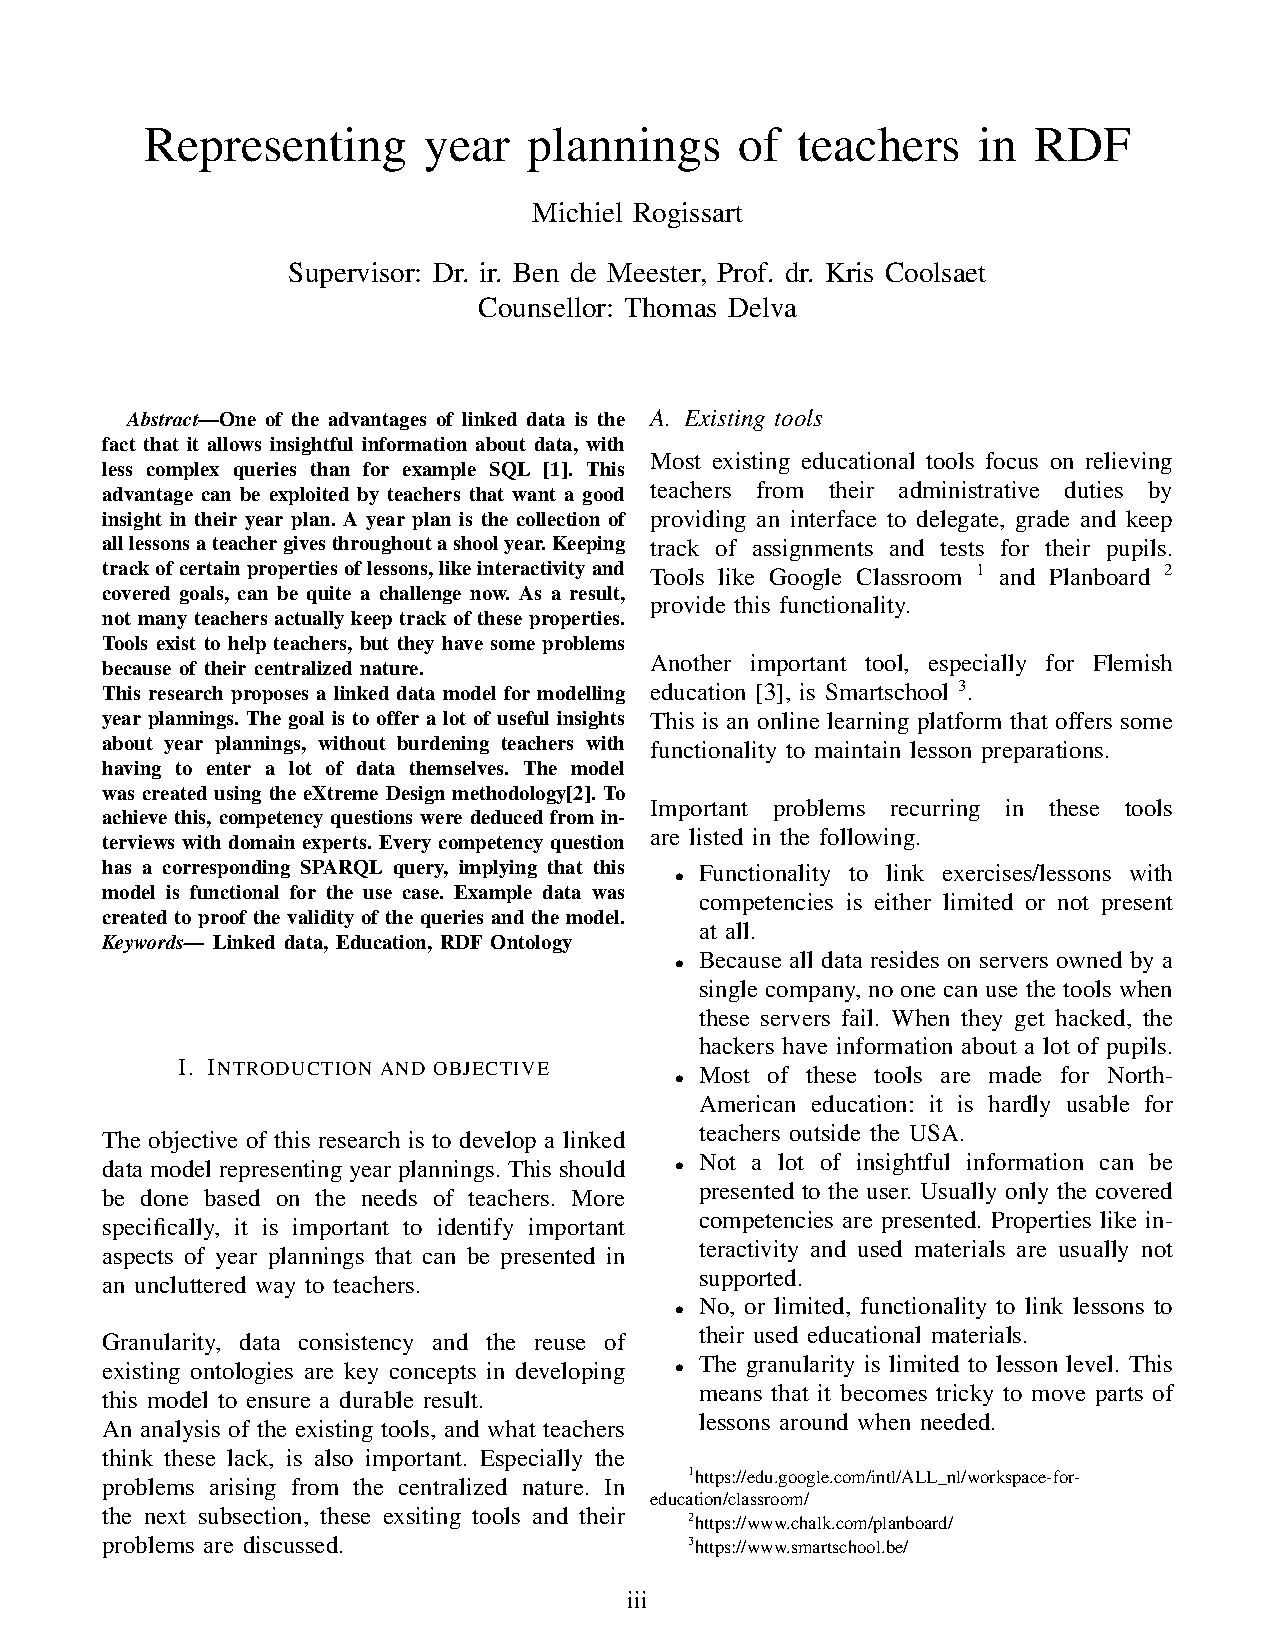
\includepdf[pages=-]{extendedabstract/extendedabstract-en.pdf}
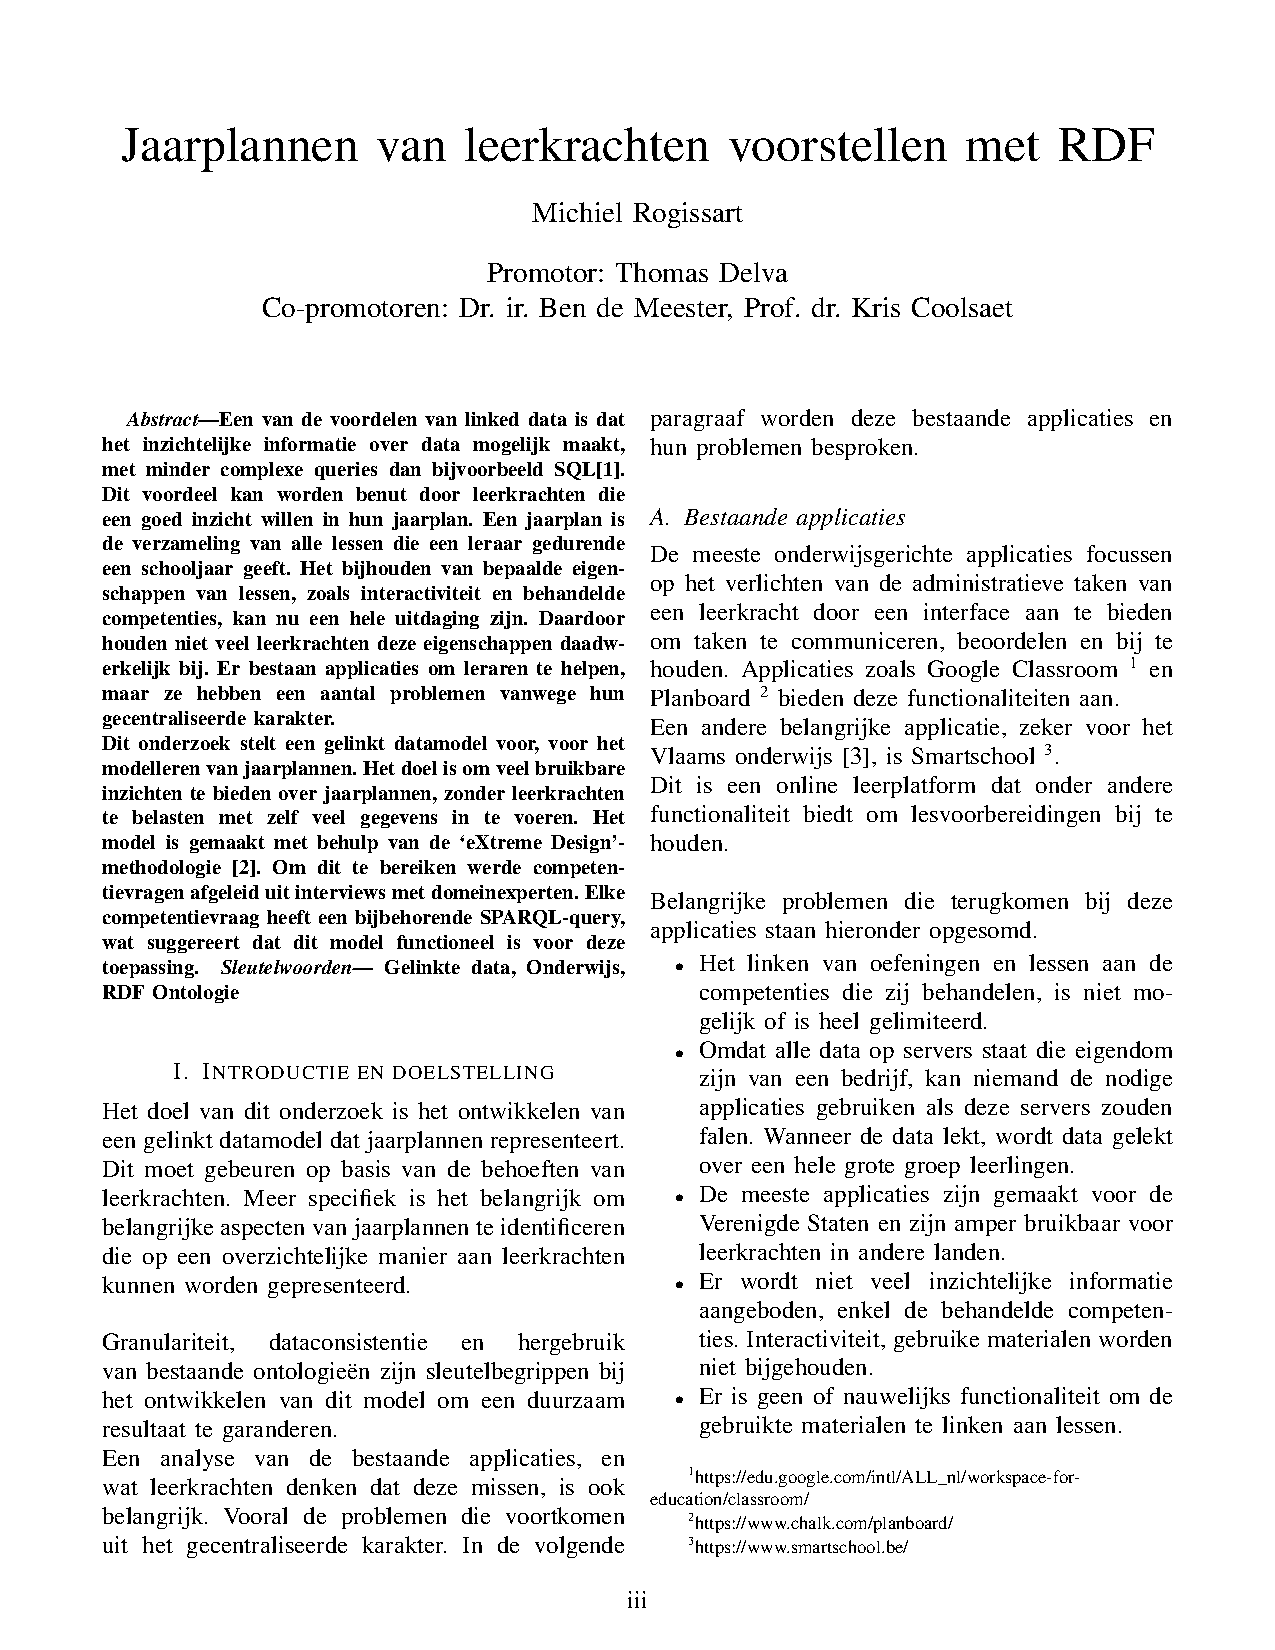
\includepdf[pages=-]{extendedabstract/extendedabstract-nl.pdf}
\newpage
\noindent A lot of data is created on the web everyday: people posting what they did, writing reviews or making their calendar for the coming week.
All this data is stored in `relational databases' which reside on computers often owned by large corporations.
A concept represented by this data, is called a resource. This can be anything from a tweet on Twitter, a laptop sold by a webshop or even a person.
When you create an account on a website, you become a resource, represented by an entry in a relational database of some company.
When you make different accounts on different websites, all these different entries represent the same resource: you.
This is because relational databases are big, structured chunks of memory in a computer.
Being `represented by an entry in a relational database', actually means being represented by some ones and zeros stored on a computer owned by someone else.\\ \\
Linked data works fundamentally different: rather than representing a resource with an entry in a relational database, it is represented by a URL.
Instead of chosing multiple usernames for multiple companies, you choose one URL for all companies. For example https://www.somedomain.com/myname, or https://firstname.lastname.com.\\
Again, everything can be represented by a url: people, books, numbers, items for sale...
Because URLs can be shared and referenced by anyone, data can be linked together.
If a laptop manufacturer provides a URL for a certain model, reviewing websites can refer to it.
The manufacturer can then write code to find all reviews referencing that particular model.\\
The link that was made, in this case between a laptop and a review, is semantic: it represents a real world relation. Namely that of someone having an opinion about a laptop.
These semantic relations (which are mostly standardized) make it easier to get complex insights in the data.\\ \\
In this paper, the advantages of linking data and retrieving complex insights are exploited in an educational context.
A data model is proposed for representing year plannings of teachers.
This would allow teachers to have insights in their lesson throughout the year with minimal input from themselves.
Because of decentralization, teachers can use data from different sources to plan their year optimally.
They could use data published by the governement to keep track of the competencies they need to cover, data published by publisher about the text books they use or even lesson preparations of colleagues.\\ \\
The model was created based on interviews conducted with teachers. This provided insights in how teachers maintain their year plannings now, and what information they're lacking about them.\\
Lessons here are considerd as a sequence of lesson phases, providing as much precision as desired.
These lesson phases can be annotated with data like the competencies they teach, which pages in which book are covered and which exercises are made.
Also links with educational taxonomies like the taxonomy of Bloom and data about the didactical method can be added. This enables teachers to offer enough variation throughout the year.\\
Not only teachers are data producers in this model. Another imporant actor are the publishers publishing text books.
They can publish data about the structure of their books: which chapters cover which competencies, which chapters belong together in a section, which exercises belong to which chapter...
Also exercises can be annotated: the difficulty, link with educational taxonomy, exercise types...\\ \\

\newpage
\noindent
\LARGE\textbf{Preface}\\

\noindent\large
De auteur geeft de toelating deze masterproef voor consultatie beschikbaar te stellen en delen van de masterproef te kopiëren voor persoonlijk gebruik. Elk ander gebruik valt onder de bepalingen van het auteursrecht, in het bijzonder met betrekking tot de verplichting de bron uitdrukkelijk te vermelden bij het aanhalen van resultaten uit deze masterproef.
\today
\section*{Word of thanks}
I thank Thomas Delva and Dr. ir. Ben De Meester (University of Ghent) for there intensive guidance throughout this thesis.
Also thanks to Prof. dr. ir. Kris Coolsaet for helping with the educational part of this research.
I'm also very thankful to the teachers that gave me some of their spare time to conduct an interview.\\ 
A special thanks to Prof. dr. ir. Ruben Verborgh (University of Ghent) for sparking my interest in linked data and help me understand the benefits.
Last but not least, I wish to thank the University of Ghent for everything I've learned there and enabling me to research this interesting topic.


\tableofcontents
\printnoidxglossaries{}
\newpage
\pagenumbering{arabic}
\setcounter{page}{1}


\maketitle

    \begin{abstract}
        The semantic web enables developers to link data from different sources to each other on a semantical level.
        This offers numerous possibilities, but these are not yet fully utilized in the educational domain.
        The purpose of this paper is to propose a data model to represent lessons and its different aspects.
        This has the goal of laying a foundation for tools that help teachers keep track of lessons and share them with each other.
        Because of the nature of linked data, these tools can offer more insightful data than traditional tools using relational databases.\\
        The model was created using the eXtreme Design methodology \cite{xd}. Interviews were conducted with teachers and these were processed into requirement stories.
        From these requirement stories, competency questions were distilled that were implemented.\\
        Granularity, consistency and reusability were the key concepts in developing the model to ensure durability.\\
        \textbf{Keywords -- Linked data, Education, RDF Ontology}
        
    \end{abstract}
    
    \chapter{Introduction}
    The goal of linked data is to link data from different sources. A data provider can provide a URI for a resource which can be used by other data providers to uniquely identify that resource. A resource can represent anything one could think of.\\
    A concrete example would be the following: a laptop manufacturer has a laptop called `ViBook'. It can provide a document on the web with URI \\ \textit{http://www.thecompany.com/vibook} with it's specifications.
    A website reviewing laptops could then publish reviews about the ViBook. It can unambiguously reference the correct model by using the URI. This website can also automatically retreive all specifications, published by the manufacturer, by fetching the associated document.
    By retreiving the specifications directly from the manufacturer, and not having to manually enter the data itself, the reviewing website has a lower risk of inconsistent or false data due to human errors.\\
    If there is a third website for selling laptops, it can also automatically retrieve the specifications directly from the manufacturer and the reviews from the reviewing website.\\
    A website for comparing laptops could combine data from the other 3 websites and also other websites with similar purposes (for example two different selling websites with different prices).\\
    Because of the URI uniquely identifying the laptop model, all data is linked to each other.\\ \\
    Representing this data is done using RDF \cite{rdf}. RDF (\textit{Resource Description Framework}) represents data using triples of the form \textit{subject, predicate, object}. The subject and predicate are always a URI, thus a resource on the web.\\
    The object can either be a URI or a literal (a string, an integer etc). The predicate defines the semantics of the relationship between subject and object and has a direction (i.e. switching subject and object gives a new triple).\\ \\
    To make this possible, standards are needed. These standards are called \emph{ontologies}. An ontology provides URIs for creating linked data describing similar concepts.\\
    A concrete example is the foaf ontology \footnote{http://xmlns.com/foaf/spec/} for representing people, organizations etc.\\
    Consider Alice and Bob, who are represented by the URIs http://mysite.com/alice and http://anothersite.com/bob.\\
    In Turtle syntax \cite{turtle}, which will be used from here on out, these URIs are notated as \textit{mysite:alice} and \textit{anothersite:bob}.
    To communicate that these people know each other, the triple (\textit{mysite:alice foaf:knows anothersite:bob}) is needed.\\ \\
    Notice how the predicate \textit{foaf:knows} is a URI to the foaf ontology. This URI leads to a document also containg linked data with RDF triples, describing the classes and predicates that can be used within the foaf ontology.\\
    Also notice how the URIs of Bob and Alice don't need to have the same domain in order to be linked.\\ \\
    When more organizations publish linked data, a web of data is created. This web is called the \textit{semantic web}.\\ \\
    Publishing data as linked data has numerous advantages. One of these is the fact that there can be more decentralization: many corporations can share and link data with eachother, eliminating the need for big corprorations with a lot of data.
    This takes away the `single point of failure': if the big corporation fails, no one can access the data. Also, when a website gets hacked, the hackers have less data that can yield security risks compared to when the big corporation gets hacked.\\ \\
    Another advantage, and the most important one for this paper, is the fact that linked data is semantic: the predicates used between subject and object relate to real world relations between the concepts they model. Because these predicates are standardized, one can perform semantic queries.
    Semantic queries, queries based on the semantics of the data rather than the structure of a database, make it easier to perform complex queries than, for example, SQL \cite{sqlvsqparql}. The query language for RDF data is called SPARQL \cite{sparql}.\\ \\
    The capabilities of linked data are not yet fully utilized in the educational domain. Studies exist on creating online learning object repositories, for example Limongelli, C. et al \cite{olap}.\\
    There are also studies on creating educational ontologies, for example Mencke, S. et al \cite{hierarchy} or Quemada, J. et al \cite{usecasebased}. There are no official releases of these ontologies or repositories in an RDF-format.\\ \\
    Because of the absence of good educational ontologies in RDF, there are no online tools that can assist the different players in the educational domain. \\ \\
    The primary goal of this paper, as explained in more detail in section \ref{subsection:goals}, is to use linked data to provide teachers with insightful data about the lessons they teach, so that tools can be created to create, maintain and share this data. \\ \\
    In this paper, the focus is on the Flemish educational system, more specifically `secundair onderwijs' (typically for pupils ages 12 through 18). The way the data is modelled can however also be used in other eduational systems, or even outside official educational systems (like workshops or refresher training).\\ \\
    Because linked data is used, teachers can use data from different sources to adequately describe their lessons: publishers can publish data bout their textbooks, governments can publish data about the required competencies, schools can publish schedules when classes occur and so on.\\
    More on this in the conclusion (section \ref{section:conclusion}).\\ \\
    The data primarly modelled in this paper is about the \textit{year plan} of a teacher. Year plannings can be described as the metadata of all lessons given troughout a school year.
    Teachers will plan their lessons based on the already given lessons, meaning that year plannings can change often throughout the year (more on this in section \ref{subsection:interviews}). \\
    The more data teachers have about the year plan, the better they are informed when planning new lessons.
    Using metadata of publishers, teachers can select relevant pages of a book for a particular lesson.
    When sufficient annotations are added, teachers can get a good overview of how many lessons are interactive, which goals are covered in which lessons, how many lessons cover a goal, where in the taxonomy of Bloom their lessons reside, and so on.

    \chapter{Goals and research questions}
    In this section, the goals of this paper are explained in more detail. The research questions that arose from these goals are also discussed.

    \section{Goals}
    \label{subsection:goals}
    The goal of this paper is to propose a data model for modelling lessons and year plannings using linked data.
    This linked data should be able to provide useful and insightful information to teachers about their year plan. What teachers deem `useful' and `insightful' is described in section \ref{subsection:interviews}.\\
    This model could form the basis of a tool for teachers to create, maintain and share data about their year plannings.\\
    Such a tool is useful because existing tools providing similar functionality but don't use linked data, have some shortcomings due to their centralized architecture (more on this in section \ref{subsection:existingtools}).
    Building such a tool using linked data instead of relational databases, could solve these problems.

    \section{Research questions}
    \label{subsection:questions}
    The research in this paper is twofold.\\
    The first part is more educational minded. The goal here is to find out how teachers keep track of their lessons throughout the year, what they already know about their year plan and what they would like to know.
    The tools already used to do this, and the problems that come with them, are also of interest. Questions arising from these goals are the following:  
    \begin{itemize}
        \item What tools do teachers use to keep track of lesson preparations throughout the year?
        \item What are the benefits and downsides of these tools?
        \item Which information about their year plan do teachers keep track of when preparing lessons?
        \item Which information about their year plan would teachers like to have when preparing lessons?
        \item Which features are interesting for a tool to maintain a year plan?
    \end{itemize}
    This is researched by interviewing teachers with some years of experience in the field (see section \ref{section:methodology}). The results are discussed in section \ref{subsection:interviews}. The existing tools and their problems are described in section \ref{subsection:existingtools}. \\ \\
    The second, and largest, part is modelling this data. This was done using the Extreme Design methodology\cite{xd} (see section \ref{section:methodology}). The used ontologies are described in section \ref{subsection:ontologies}.
    Questions arising from this goal are the following:
    \begin{itemize}
        \item Which ontologies already provide resources to describe year plannings and lessons?
        \item How can we translate the information teachers want about their year plannings to concrete questions that can be answered?
        \item How can we model this data so that these concrete questions can be answered?
        \item Which SPARQL queries are needed to answer these concrete questions?
        \item How can we keep the data consistent?
    \end{itemize}
    The resulting data model is discussed in section \ref{section:datamodelling}. The data made to test the model and the SPARQL queries are described in section \ref{section:data}.

    \chapter{State of the art}
    In this section, the state of the art is discussed. The first subsection discusses existing tools that can be used to maintain year plannings. These tools are shortly discussed and the problems they have are explained more in depth.\\
    The ontologies used in the model are discussed in the next subsection. The core concepts on which this model relies upon are explained.\\
    Lastly, some relevant data sources are discussed. These sources contain data about the Flemish educational system that are used in the data created to test the model.
    \section{Existing tools}
    \label{subsection:existingtools}
    Most existing educational tools focus on relieving teachers from their administrative duties by providing an interface to delegate, grade and keep track of assignments and tests for their pupils.
    Tools like Google Classroom\footnote{https://edu.google.com/intl/ALL\_nl/workspace-for-education/classroom/} and Planboard\footnote{https://www.chalk.com/planboard/} provide this functionality. These tools have some issues that have to be solved:
    \begin{itemize}
        \item Functionality to link exercises/lessons with competencies are either limited or not present at all.
        \item It is hosted by private companies, which means that all information resides on their servers. This imposes some security risks: leaking this database gives hackers a lot of information about a lot of pupils. When these servers fail, no one can access the data or the tools that are needed.
        \item Most of these tools are made for North-American education: it is hardly usable for teachers outside the USA.
        \item There is not a lot of functionality to generate overviews. Most of the time, only an overview of the covered goals can be generated. There are different overviews that can be of use as well (seee section \ref{subsection:interviews}).
        \item There is no or limited functionality to link lesson prepartions to the used educational material.
        \item The granularity is mostly on lesson level. There is no way to split lessons into phases that can be moved across lessons.
        \item Teachers need to enter most of the information themselves and cannot rely on data created by other people.
    \end{itemize}
    Having said this, there is one tool that is very important in Flemish schools: Smartschool\footnote{https://www.smartschool.be/}.
    This is an electronic learning environment used by over 90\% of Flemish schools \cite{destandaard}. It offers a lot of functionality: gradebooks, uploadzone, a student tracking system, sending and receiving messages within the school, sharing resources with other schools etc.
    Smartschool offers very limited functionality to make lesson preparations: a short paragraph of text describing the lesson, nothing more. There is an optional module to make year plannings and link them with the lesson preparations. You can specify the goals you cover and group lesssons in lesson series.
    This module, however, lacks a lot of functionality: there is no way to link lessons to the used educational materials, lessons cannot be shared and some important metadata is missing (difficulty, target group, competencies to be covered etc.)
    An important part of the missing data about lesson preparations in this tools, is data about the \textit{didactical method}. A didactical method is the manner in which subject matter is taught.\\
    It has important characteristics, such as: interactivity, the nature of the lesson (repetition, introducing new subject matter...) etc. More on the important characteristics of didactical methods can be found in the conclusions of the interviews (section \ref{subsection:interviews}).\\ \\
    The last important feature that Smartschool, and the other tools, are missing, is the ability to move parts of lessons to different lessons.\\
    This is a problem of granularity: these tools only have descriptions of entire lessons, moving parts of these lessons to other lessons (for example because there was not enough time) is necessary for optimal flexibility.
    The solution for this does not reside in linked data, but it will be an important part of the model.

    \section{Ontologies}
    \label{subsection:ontologies}
    Some standards and ontologies for the educational domain are already developed.
    IEEE released a standard \cite{ieeelom} concerning LOM (Learning Object Metadata). These standards are implemented by Schema.org \cite{schema} and DC (Dublin Core) \cite{dc}.
    It provides a very basic, but quite complete, ontology for handling learning objects. Most research on LOM build further on this ontology. For example \cite{usecasebased} introduces an extra
    distinction to categorize better: Educational Activities and Educational Material. There is no distinction between these two concepts in the original ontology. \\
    The Flemish goverment released a standard vocabulary to be used with these ontologies\cite{pubelo} \cite{pubelovoc}. \\ \\
    There is also some research done about representing didactical methods with ontologies. Even though this will not be a focus of this research, the properties of didactical methods should be modelled because of their close relations to lesson preparation and the insightful data it could give.\\
    The interviews should clearify which properties teachers find useful to keep track of.\\
    A resuable and sustainable ontology for describing didactical methods was proposed by Mencke, S. et al \cite{hierarchy}.\\ \\
    Some important concepts of schema.org and DC used in this model are explained in the following subsections.

    \subsection{Schema.org}
    The core class of this ontology for the model is \textit{CreativeWork}. This models any kind of creative work like books, movies, photographs but also lessons.\\
    This has a subclass \textit{LearningResource} which is meant to be used in conjunction with other, more concrete, classes (like Book or Movie).\\
    CreativeWork instaces can be part of each other by using the \textit{isPartOf} property, which is useful to introduce some kind of hierarchical structure between lessons.\\
    There are also some very useful properties that relate to education like \textit{teaches}, \textit{assess}, \textit{interactivityType} etc.\\ \\
    The classes \textit{DefinedTerm} and \textit{DefinedTermSet} are also very important for this model. DefinedTerms are mainly used to link the model with data sets that are useful, but not part of, the data modelled here.\\
    A good example are competencies: these are communicated by the government through URIs. The government chooses which ontology it uses for this.
    Representing a competency as a DefinedTerm containing a URI to the data of the government, makes it possible to model competencies without relying on the ontology used by the government. URIs can then be dereferenced to get the data of the government.\\
    DefinedTermSets can be used to group competencies together based on domain or educational level. This makes it easy to find all competencies required for a certain level a pupil is in.\\ \\
    Schema also offers classes to model documents and books. These do not offer the necessary properties to adequatly model them in an educational context. That's why DC is used for the educational materials.\\
    The class \textit{DigitalDocument} of Schema is used for documents describing lessons (see section \ref{subsubsection:descriptions}).

    \subsection{Dublin Core}
    The Dublin Core standards are used when modelling educational material such as text books and teacher made material. More specifically the bibo ontology \cite{bibo}.\\
    The most important class used is \textit{Document}, because all other used classes inherit from it.\\
    It contains properties to describe chapters, sections and excerpts. This offers a high level of granularity to accurately describe which part of the material is relevant for the lessons.
    There are also a lot of properties for metadata concerning copyright.

    \section{Data sources}
    The Flemish government released two data sources that are of interest for this research.\\
    The first one is a skos dataset describing the learning goals, educational levels and curricula imposed by the Flemish government \cite{ilearnskosmos}, created within the i-Learn project \footnote{https://www.i-learn.vlaanderen/}. 
    Subjects were also added to this dataset, but the government does not decide which subjects are taught at schools. Only the goals that have to be covered. \\
    In addition to the skos dataset, the Flemish government has a regular JSON-api \footnote{https://onderwijs-vlaanderen-portaalov.apigee.io/apis} with some basic information about the educational structure.
    All information from this JSON API can also be found in the skos dataset. \\ \\
    Then there is one last project by the Flemish government which can be of use: Klascement \footnote{https://www.klascement.net/}. This is a learning object repository (LOR) with a lot of educational materials shared by teachers.
    This does not use RDF but does yield some semantic data. It's more about learning materials rather than lesson preparations, but still can be of great inspiration. 
    
    \chapter{Methodology}
    \label{section:methodology}
    In this section, the methodology used to create the model is discussed.\\ 
    It is based on the Extreme Design methodology \cite{xd} and consists of 2 phases: a preparation phase and an implementation phase.
    \section{Extreme Design}
    The Extreme Design methodology \cite{xd} is a methodology specifically created for ontology design in teams. It is based on pair design and offers a road map on designing ontologies. This roadmap is shown in figure \ref{fig:xd-diagram}.
    \begin{figure}
        \caption[Extreme Design roadmap]{Extreme Design roadmap as mentioned in \cite{xd}}
        \centering
        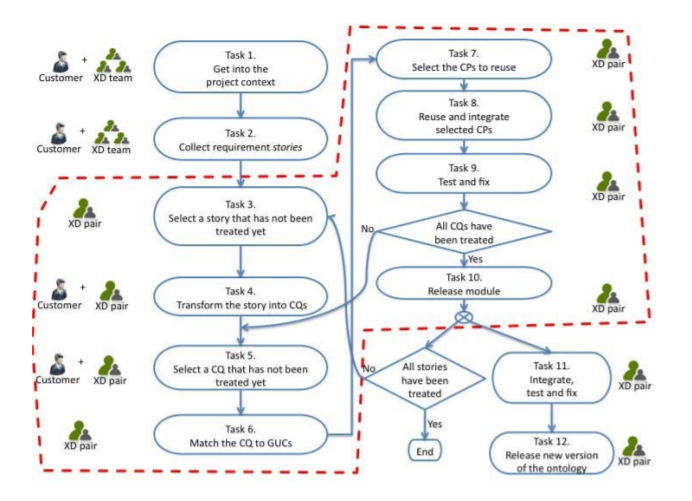
\includegraphics[scale=0.75]{xd-diagram.PNG}
        \label{fig:xd-diagram}
    \end{figure}
    In the preparation phase, interviews are conducted with domain experts. These are people that know what the consumer of the data want.
    These interviews are then processed into \textit{requirement stories}. These are concrete stories of how one might use the data. 
    This is closely related to use cases, but are less narrow. The requirement stories can be found in the GitHub repository of this research \cite{repo}. \\
    An example of a requirement story is ``A teacher would like to keep track of which goals are covered in which lessons.'' \\
    Out of these requirement stories, \textit{competency questions} and \textit{contextual statements} are ditsilled. Competency questions are questions one might ask about the data. An example of such a competency question could be: ``How many lessons did I spend on goal x?".\\
    Contextual statements are facts about the represented concepts as stated by the domain experts. An example is `` A lesson covers 0 or more competencies''.\\
    The competency questions and contextual statements for this research can also be found in the repository \cite{repo}.
    The ones concerning didactical methods and taxonomies can be found in appendix \ref{chap:appendix-cq} \\ \\
    The following section describes the interviews in more detail, along with the conclusions drawn from them.

    \section{Interviews}
    \label{subsection:interviews}
    Three interviews were conducteed to find out what teachers find useful in a tool to make lesson preparations and year plannings.
    Two of those were teachers informatics in a traditional school. The third teacher was a language teacher in a method school.
    Being a method school, the latter has a very clear didactical method that they use for all pupils (mostly the ADI-method and the digital method). The way they teach is fundamentally different from the other two teachers.\\ \\
    Despite these differences, one thing was clearly the same for all these teachers: they see their year plan as a dynamic instrument that changes as the year progresses.
    This means that it is important to link lessons to the agenda of the teachers and maintain a high degree of flexibility in reordering the lessons, for example when a small part of a lesson moves to the next because there is not enough time.
    However, it is important that teachers are still able to prepare lessons without having to plan them immediately.
    For example: if a teacher plans on spending 3 weeks on a particular chapter, it should be possible to lay the foundation of this whole series of lessons easily without having to worry when these lessons will be taught.
    A good solution for this is to model time and place independent lessons which can later be linked to the agenda and easily moved around.\\ \\
    Another thing all interviewees agreed upon, is that it is useful to track data about learning taxonomies.\\
    These are taxonomies to indicate on which level one possess the subject matter. The most important one is the revised taxonomy of Bloom.\\
    It will be important to model this as well, especially since this is incorparated in the Flemish educational system.\\ \\
    There are of course some differences between the interviewees. The informatics teachers use their own textbook since there are not many textbooks available for informatics.
    They rely heavily on past experience and know how they want to teach a particular unit and how much time they spend on it. This means that it is important
    that teachers can link their own textbooks to their lessons (as well as textbooks bought from publishers).
    The language teacher also has her own textbook because it is very much intertwined with the didactical method the school uses.
    The difference here is that the lessons are given by 2 teachers, so they have to work together. Their lessons are also constantly evaluated for future years.
    This means that it is very useful for them to be able to enter some thoughts about their lesson after they've taughed it.
    The biggest difference between the traditional school and method school is, not surprisingly, the way they think about didactical methods.
    Whereas the informatics teachers don't really think about which didactical methods they use, the method school strives to incorprate appropriate didactical methods.
    A big difficulty will be to adequately describe a didactical method: it is important to make the necessary distinctions, without having a jungle of didactical methods that only differ slightly.
    Distinctions this teacher found usefull are:
    \begin{itemize}
        \item Active or passive
        \item Strongly, weakly or not steering
        \item If pupils physically move or not
    \end{itemize}

    \chapter{Data modelling}
    \label{section:datamodelling}

    The resulting model is discussed in this section. To maintain an overview, this was split up into different parts:
    \begin{itemize}
        \item Competencies, credentials and educational levels (section \ref{subsection:compmodel})
        \item Lessons, lesson phases and year plannings (section \ref{subsection:yearplans})
        \item Courses, subjects and classes (section \ref{subsection:courses})
        \item Course material and exercises (section \ref{subsection:coursematerial})
        \item Didactical methods and educational taxonomies (section \ref{subsection:taxonomies})
    \end{itemize}

    The last subsection (subsection \ref{subsection:results}), motivates why the problems stated in section \ref{subsection:existingtools} are solved using this model.

    \section{Competencies}
    \label{subsection:compmodel}

    The competencies are completely modelled using Schema.org. A UML diagram is found in figure \ref{fig:uml-comp}.\\

    \begin{figure}[h]
    \caption{Modelling of competencies}
    \label{fig:uml-comp}
    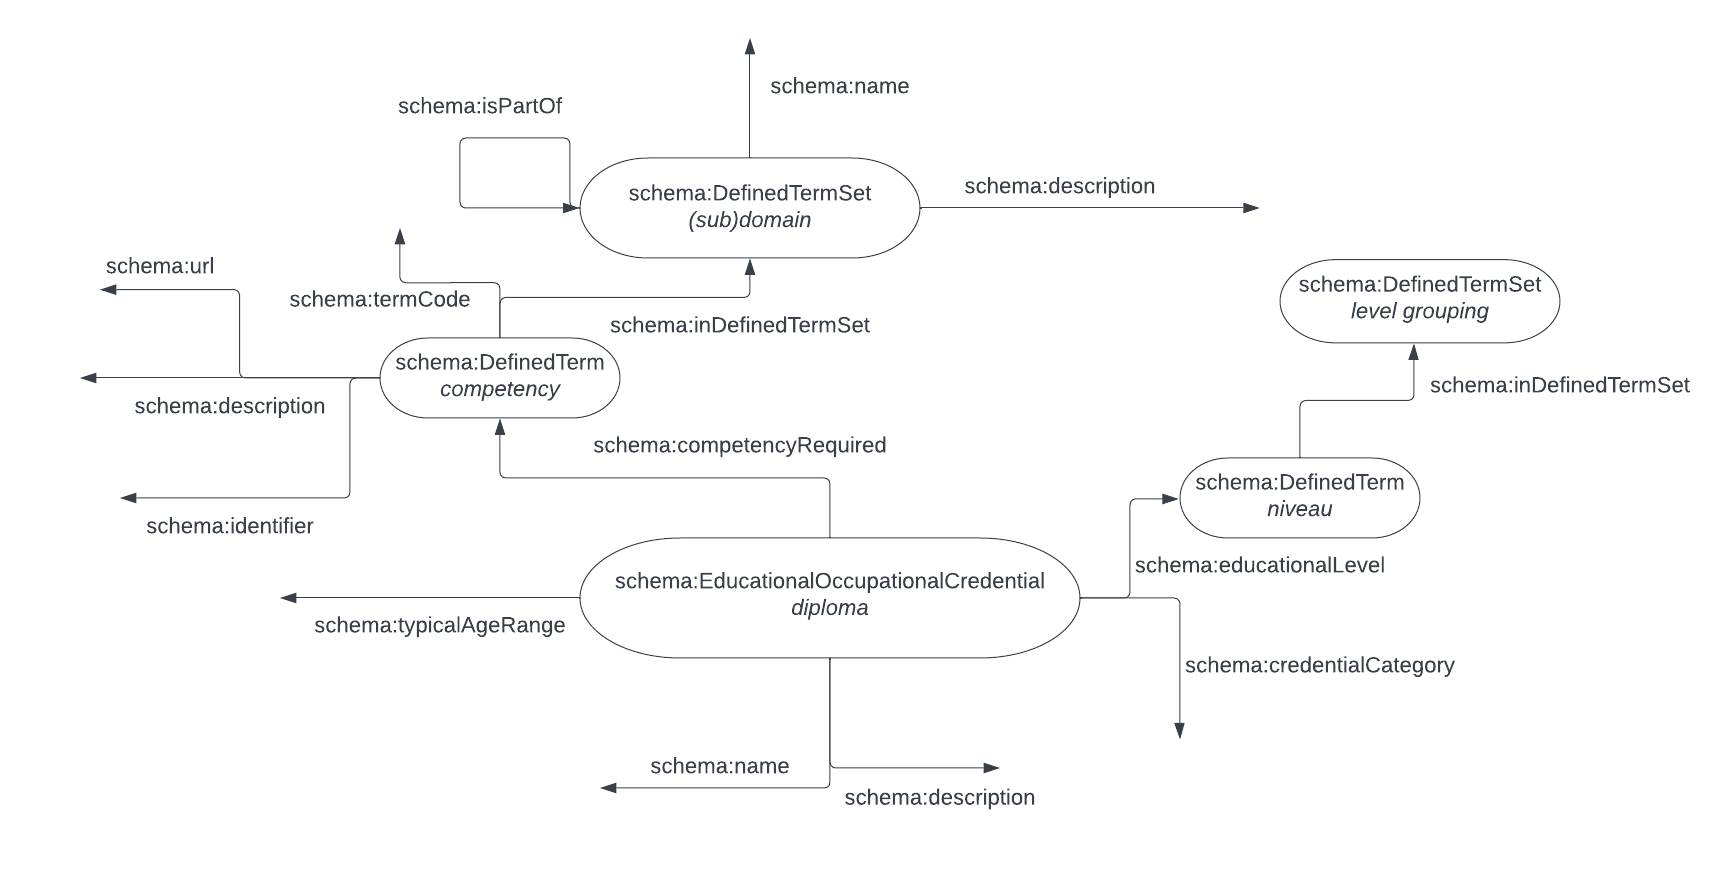
\includegraphics[scale=0.5]{uml-competencies.png}
    \end{figure}
    \noindent As previously mentioned, competencies are modelled using the \textit{schema:DefinedTerm} class.
    A link to the data set of the government can be preserved by keeping the original URI (as done here, see section \ref{subsection:comp}) and/or by using the property \textit{schema:URI}. \\
    Other important properties are the following:

    \begin{itemize}
        \item \emph{schema:description} is a string representing the formal definition of the competency.
        \item \emph{schema:termCode} is a (textual) code that uniquely identifies the competency across all competencies. This can also be an integer, but the Flemish government uses strings.
        The documentation of schema.org states that the termCode should only uniquely identify the DefinedTerm within the set it belongs to. In this case, it is feasable that there is a set containing all competencies.
        Thus, it's a good practice to use an identifier that is unique across all competencies.
        \item \emph{schema:identifier} an identifier that should be unique across all DefinedTerms.
        \item \emph{schema:inDefinedTermSet} indicates that a competency is part of a set. Sets can be created for domains, subdomains, levels or a combination. Domains and subdomains are discussed in the next section.
    \end{itemize}
    DefinedTerm is a good class for representing competencies as it makes it easy to use them without having to rely on the ontology used by the government (or other official organization).\\
    It is clear that schema.org expects competencies to be modelled like this when looking at the documentation \cite{schema} for the \textit{schema:teaches} and \textit{schema:assesses} properties. These have a DefinedTerm as range and it is clear that semantically, this corresponds to competencies.

    \subsection{Competencies and (sub)domains}

    Competencies can be grouped together in domains and subdomains. These groupings are typically defined by a government or other official organization.\\
    These domains are modelled with the schema:DefinedTermSet class. A subdomain is also a schema:DefinedTermSet which can be part of a broader set representing the domain.
    Important properties are \textit{schema:name}, representing the name of the (sub)domain, and \textit{schema:description}, providing an official description of the (sub)domain.\\
    To model subdomains that are part of a broader domain, \textit{schema:isPartOf} is used.\\ \\
    Semantically, a domain is nothing more than a set of competencies that are closely related. Using a DefinedTermSet for this is thus the most logical option.

    \subsection{Educational levels and credentials}

    Education is typically split up into different levels between which a pupil must choose, leading to different credentials. Some levels focus more on theoretical competencies, where other levels focus more on skills.\\
    An educational level is modelled using the schema:DefinedTerm class. Important properties are the following:
    \begin{itemize}
        \item \emph{schema:name} represents the official name of the educational level.
        \item \emph{schema:alternateName} is an optional alternate name for the same educational level.
        \item \emph{schema:typicalAgeRange} models the typical age of pupils in this level.
        \item \emph{schema:inDefinedTermSet} indicates that an educational level is part of a grouping of educational levels (see further).
    \end{itemize}

    \noindent Just like competencies, educational levels are defined by the government or other official organization and thus will most likely have a URI in the domain of that government/organization.
    The documentation for \textit{schema:educationalLevel} has DefinedTerm as range, which suggests that this class is the right class to model educational levels.
    Educational levels can be grouped together by age range and/or focus (theoretical or skill) which can also be formally defined by a government or other official organization.\\
    These groupings are modelled with \textit{schema:DefinedTermSet} that also have the properties \emph{schema:name}, \emph{schema:alternateName} and \emph{schema:typicalAgeRange}.\\
    Groupings can be grouped together even further using \emph{schema:isPartOf}.
    The reason behind this choice is analogue to domains and (sub)domains as discussed in the previous section.\\ \\
    When a pupil completes an educational level, a credential is typically awarded.
    These are modelled using the \emph{schema:EducationalOccupationalCredential} class. Important properties are the following:

    \begin{itemize}
        \item \emph{schema:name} represents the official name of the credential.
        \item \emph{schema:typicalAgeRange} is the typical age of pupils in the process of completing this credential.
        \item \emph{schema:credentialCategory} is a string or schema:DefinedTerm representing the type of credential (certificate/diploma...).
        \item \emph{schema:competencyRequired} indicates which competencies need to be acquired to acquire the credential.
    \end{itemize}
    In the documentation of this class, it says that EducationalOccupationalCredential represents ``An educational or occupational credential. A diploma, academic degree, certification, qualification, badge, etc., that may be awarded to a person or other entity that meets the requirements defined by the credentialer.''.\\
    This is thus the best choice to model credentials.\\ \\
    The value of the property \textit{schema:credentialCategory} is a literal. This was chosen over a \textit{schema:DefinedTerm} because this has an official vocabulary.\\
    It is not expected that the government will provide a URI representing differen categories, thus a literal was chosen.

    \section{Lessons, lesson phases and year plannings}
    \label{subsection:yearplans}

    Lessons are modelled using Schema.org in union with self defined classes (the ontology for this is called myont). A UML diagram is found in figure \ref{fig:uml-lesson}.\\
    It is important to mention that the lessons that are discussed here, are \textbf{time and place independent}. They represent an idea of a lesson, rather than a lesson that is given at a certain time, in a certain place.
    Lessons can then be linked to classes, which are time and place dependent. See section \ref{subsection:courses}.\\

    \begin{figure}[h]
    \caption{Modelling of lessons}
    \label{fig:uml-lesson}
    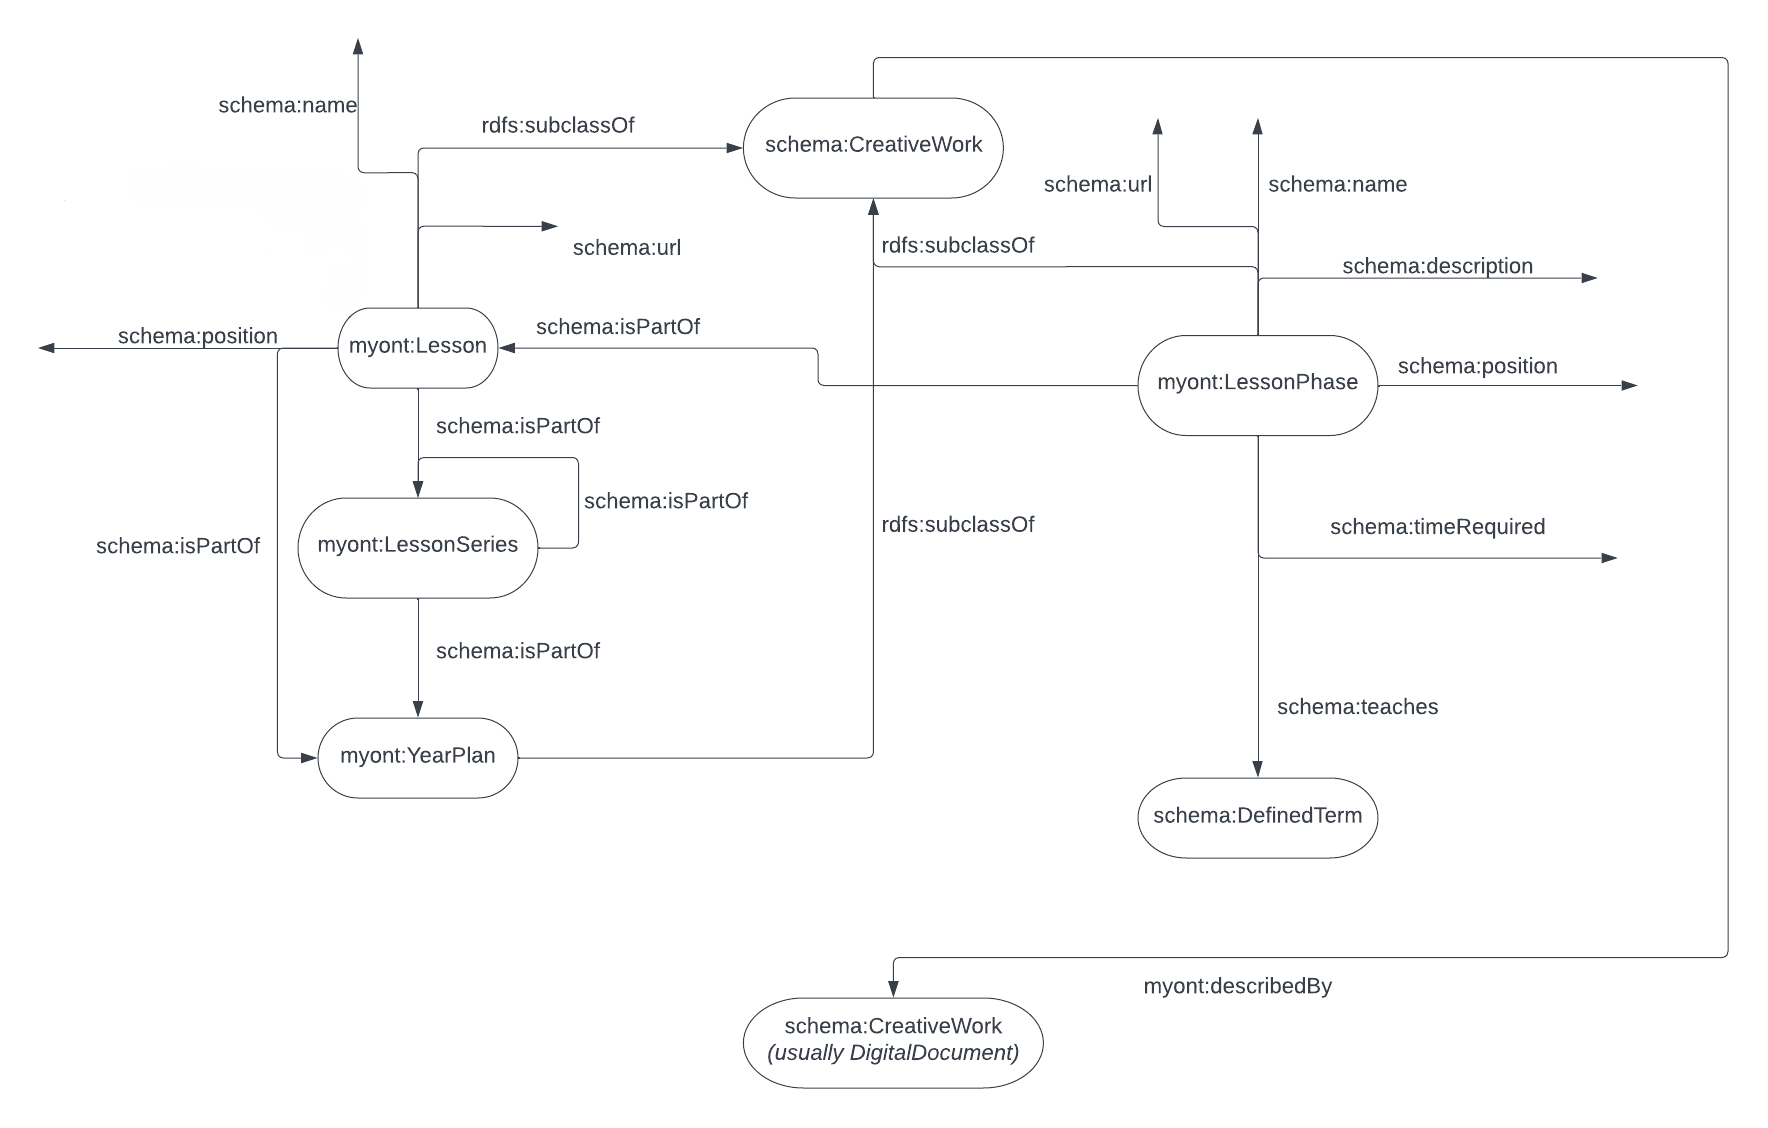
\includegraphics[scale=0.5]{uml-lessons.png}
    \end{figure}
    Important properties of the \textit{myont:Lesson} class are the following:

    \begin{itemize}
        \item \emph{schema:name} represents the name of the lesson, typically given by the teacher entering the data.
        \item \emph{schema:isPartOf} is used to build the hierarchy. Lessons are either part of a lesson series or a year plan. More on the hierarchy in \ref{subsubsection:hierarchy}.
        \item \emph{schema:position} indicates the position of the lesson within the lesson series or the year plan.
    \end{itemize}
    The reason custom classes where introduced, rather than completely depending on Schema.org, is to easily distinct lessons from lesson phases, series and year plannings. All these concepts could be modelled using CreativeWork and its subclasses, but distinguishing between them becomes harder.
    To achieve this using only Schema.org, one should look at how far a resource is in the hierarchy (the hierarchy is discussed in more detail in section \ref{subsubsection:hierarchy}).\\
    By providing different classes for these concepts, one could distinguish between them using the \textit{rdf:type} property, which will allow less complex SPARQL-queries.

    \subsection{Lesson phase}
    A lesson phase is the smallest unit to represent lessons. It represents an as small as possible, coherent part of a lesson. An example of a lesson phase could be explaining a mathematical proof, or solving an exercise.
    Like all other classes in myont concerning lessons, this class is a subclass of schema:CreativeWork. Important properties are the following:

    \begin{itemize}
        \item \emph{schema:name} represents the name of the phase, given by the person that enters the information (typically a teacher) or that is automatically generated.
        \item \emph{schema:timeRequired} is an estimation of how long this phase takes. This estimation is typically done by the teacher entering the data.
        \item \emph{schema:description} is a very short description of the lesson phase. This should not contain a full, extensive, description of the phase. Full descriptions can be provided using digital documents (see section \ref{subsubsection:descriptions}).
        \item \emph{schema:teaches} points to a competency that is taught in this lesson phase. The number of competencies taught in a lesson phase should be as small as possible
        \item \emph{schema:position} indicates in which order the lesson phases of the lesson should occur.
        \item \emph{myont:describedBy} is used to point to a digital document with a full description of how the phase should be taught. See section \ref{subsubsection:descriptions} for more details
    \end{itemize}
    Introducing the \textit{myont:LessonPhase} class eleviates the problem of granularity: lesson phases can now be moved around lessons to enable a high degree of flexibility when building year plannings.\\ \\
    It is important to mention that two lesson phases belonging to different lessons, are by definition different phases. Even if the content is exactly the same.\\
    This is needed because it would otherwise be harder to define the position of the phase within the lesson.

    \subsection{Building year plannings with lesson phases}
    \label{subsubsection:hierarchy}
    As mentioned before, different lesson phases in a particular order form a lesson. All myont:LessonPhase instances thus should have the \textit{schema:isPartOf} property with a \textit{myont:Lesson} as object.\\
    These lessons can be grouped together in a lesson series. Lesson series are lessons in a particular order that have coherent subject matter. For example a math teacher could make a lesson series for all algebra lessons, one for all geometry lessons and so on.\\
    Lesson series can be part of other lesson series to provide optimal flexibility. In a lesson series with all geometry lessons, one could make a series of lessons about Pythagoras Theorem for example.\\ \\
    Lesson series are then further grouped together into a year plan using \textit{myont:YearPlan}. Usually, one year plan is made for every school year and every group of students.\\ \\
    Note that lessons are not necessarily part of a lesson series (as opposed to lesson phases which are always part of a lesson), but will always be part of a year plan.\\
    If a teacher prepares a lesson about pi on pi day for example, this is not part of any series. It is a lessons that stands on its own and thus is directly part of a year plan.\\
    Another reason for this high level of flexibility is that not all teachers are eager to group their lessons into lesson series. In theory, one does not need \textit{myont:LessonSeries} to have a good year plan, but it can be useful to maintain an overview (depending on the person creating the data).

    \subsection{Flexible descriptions}
    \label{subsubsection:descriptions}
    Teachers should be flexible in the way they describe their lesson phases, lessons and so on. Some teachers don't mind typing an extensive, marked up, description of every phase. Other teachers only want to describe lessons.
    It can also be that a full lesson series is described in one document, for example when an external organization offers these documents.\\
    That's why \emph{myont:LessonPhase}, \emph{myont:Lesson}, \emph{myont:LessonSeries} and \emph{myont:YearPlan} all have a \emph{myont:describedBy} property with a \emph{schema:CreativeWork} as value.
    This will usually be a \emph{schema:DigitalDocument}, like a MarkDown or HTML document, but it can be any creative work. It is important to use the \emph{schema:encodingFormat} to mention the MIME type of the document.\\ \\
    Decoupling the full description of the phase from the RDF-data gives teachers more options to describe the phases. It also allows them to reuse documents they've already made, rather than having to copy paste everything when they start using the tool.

    \section{Courses, subjects and classes}
    \label{subsection:courses}
    Courses, subjects and classes are used to bind lessons to temporal data. The UML diagram is found in figure \ref{fig:uml-courses}. The different concepts are discusses in following subsections.\\

    \begin{figure}[h]
        \caption{Modelling of courses}
        \label{fig:uml-courses}
        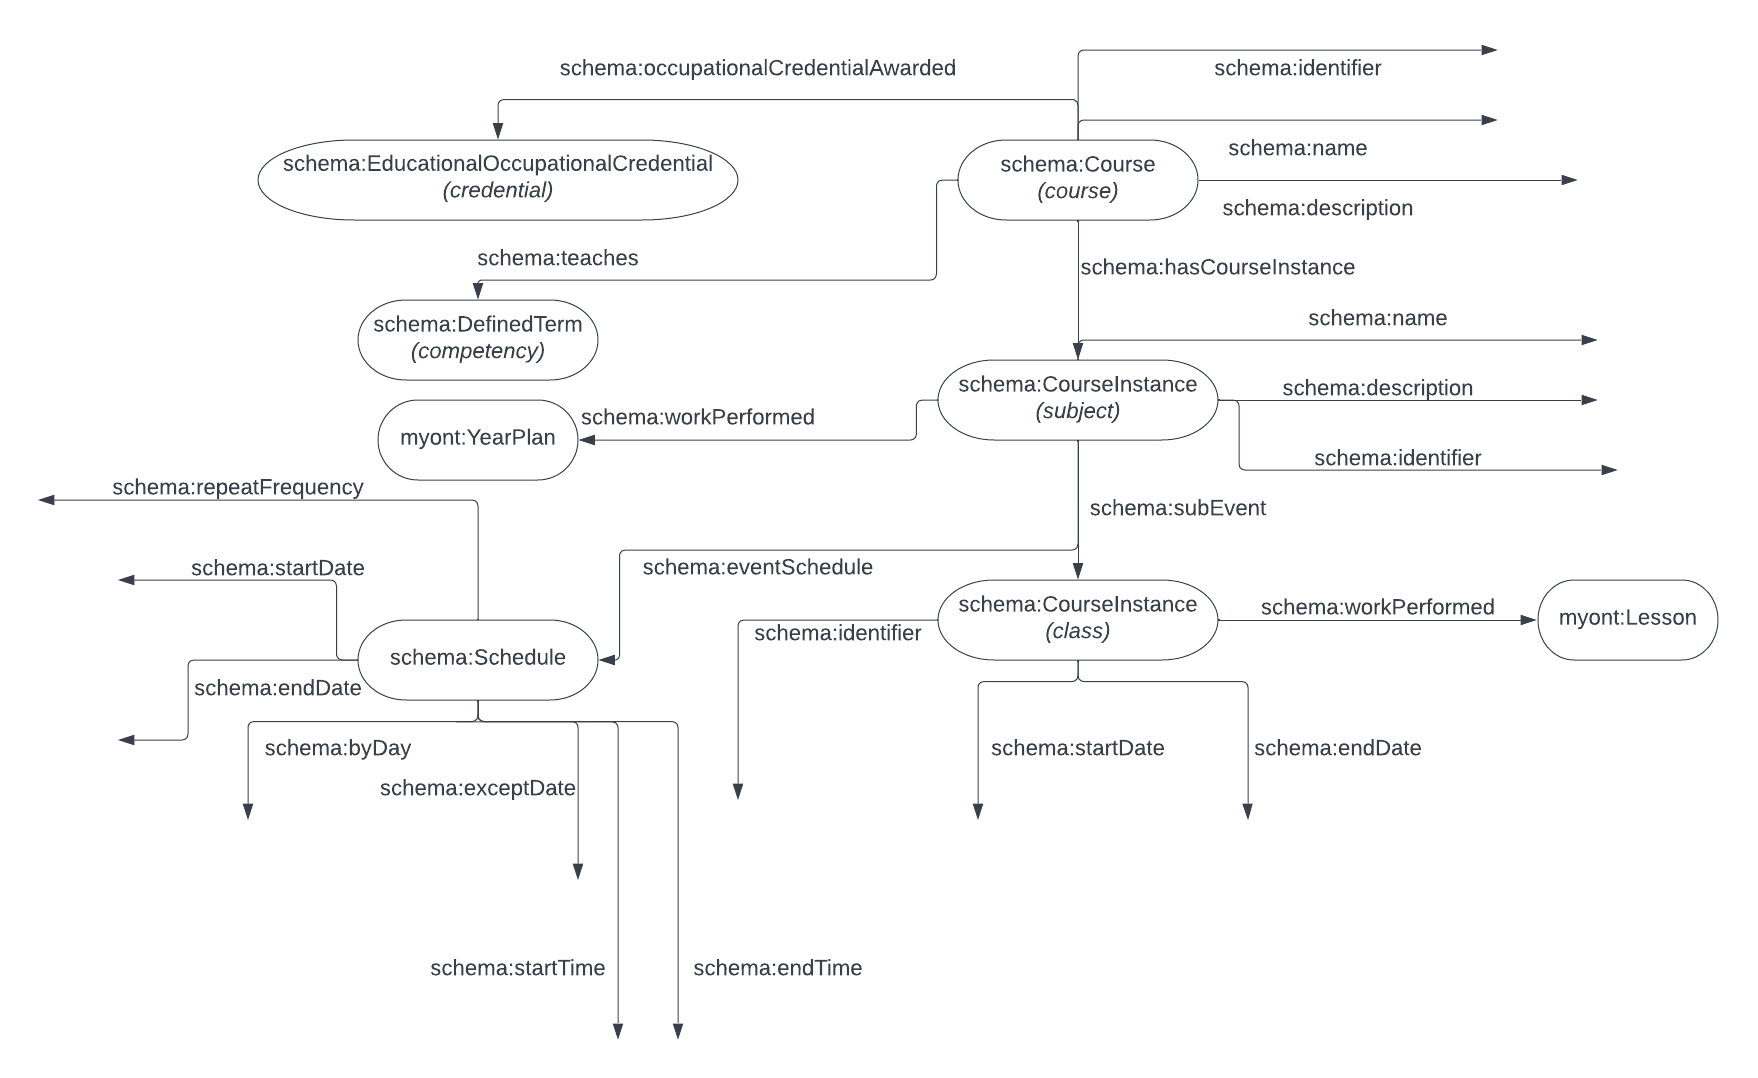
\includegraphics[scale=0.5]{uml-courses.png}
    \end{figure}
    \noindent These classes are used to bind lessons to a time and place. The most important difference is that this data is created by a school, whereas the data about lessons is created by teachers.\\
    It is the school that decides which competencies are grouped together in a single course, but it is the decision of the teacher how these competencies are taught.

    \subsection{Course}
    A course is a set of competencies, that have to be acquired for a specific credential, that are taught by the same teacher to the same group of pupils within the same school year.
    This is modelled using the \textit{schema:Course} class.\\
    This data does not contain temporal or spatial data, but gives more information on how the compentencies for a certain credential are split up. Schools often get some degree of freedom when deciding when the competencies are given.
    When a school decides to change this, a new course should be made. If this doesn't change across school years, the same course can be kept.\\
    In flemish education, competencies are grouped in groupings of 2 years. The school can decide which competencies are given in which year. This is a good example of when this is useful.
    If schools decide to share this information with each other, they can get inspired by how other schools decided to do this.
    Important properties of this class are the following:
    \begin{itemize}
        \item \emph{schema:occupationalCredentialAwarded} points to the credential of which this course is part of. 
        Typically all courses that have the same credential as object need to be finished in order to acquire the credential.
        \item \emph{schema:teaches} indicates a competency that has to be acquired to fulfill the course.
        \item \emph{schema:identifier} is an identifier chosen by the school. This should be unique across all courses, even if they don't belong to the same credential.
        \item \emph{schema:name} represents the name as communicated to the pupils. For example ``Math", ``Math 3rd year".
        \item \emph{schema:description} is a short description of the course. 
        \item \emph{schema:hasCourseInstance} indicates a subject that teaches this course (see next section)
    \end{itemize}
    This class is needed because it can be linked to a credential using the property \textit{schema:occupationalCredentialAwarded}. This property has Course as domain.

    \subsection{Subject}
    \label{subsubsection:subject}
    A subject is a course with temporal data. Typically, there will be a new subject for every school year. It is modelled using \textit{schema:CourseInstance}.
    The temporal data includes start and end date of the subject and the schedule (when the classes occur).
    Important properties are the following:
    \begin{itemize}
        \item \emph{schema:name} is the name of the subject as chosen by the school and communicated to the pupils. Examples are ``Math'' or ``Math 3rd year 2021-2022''. This can be the same as the name of the course, but doesn't have to be.
        \item \emph{schema:description} is a short description of the subject.
        \item \emph{schema:identifier} is a unique identifier for this subject. This should be unique across all subjects (not only subjects of the same course).
        \item \emph{schema:workPerformed} indicates a \textit{myont:YearPlan} is given within this subject. Only one year plan can be given within a subject.
        \item \emph{schema:subEvent} indicates a class is part of this subject. More on classes in the next section.
        \item \emph{schema:eventSchedule} indicates when classes of this subject occur. Below is more information on how to model schedules using schema.org. 
    \end{itemize}
    To model schedules, the \textit{schema:Schedule} class is used. The properties used to achieve this are the following:
    \begin{itemize}
        \item \emph{schema:startDate and schema:endDate} indicate the start and end date of the subject. This is typically the start and end of the school year, but not necessarily (see further).
        \item \emph{schema: startTime and endTime} indicate the start and end time of the class.
        \item \emph{schema:byDay} indicate on which day(s) classes occur. Schema.org provides URIs for weekdays.
        \item \emph{schema:exceptDate} indicate that there is exceptionally no class on this date. This could be because of a holiday or extracurricular activities like a school trip.
        \item \emph{schema:repeatFrequency} will typically be ``P1W", indicating a class occurs every week. Other values are possible, for example when a class only occurs every 2 weeks. 
    \end{itemize}
    Modelling schedules with schema.org can be done in different ways. A different entry was made for every class in the week, even when two classes fall on the same day or two classes on different days start at the same hour.\\
    One could also make different schedules between school vacations, as schema.org only provides functionality to exclude particular dates, and not a continous set of dates (for example 2 weeks of vacation). 
    Vacations are not modelled in this ontology as this is more about school structure rather than keeping track of lessons, which is not within the scope of this research. \\ \\
    The main reason to decouple courses from subjects is because of the schedule: while it is useful to represent the schedule in RDF, it does not make sense to link the schedule to one class.\\
    Because no schedule can be attached to \textit{schema:Course}, this is the best way to do this.
    The data about the schedule can be used to generated classes for every class that is taught throughout the year. Example code on how to this can be found in the GitHub repository \cite{repo}.\\
    More information on these scripts in section \ref{section:data}.

    \subsection{Classes}
    A class is a lesson that is given at a certain time, in a certain place. The place itself is not modelled as this is more part of the school structure.\\
    The term `class' is used to distinguish this from the lessons in subsection \ref{subsection:yearplans}, which contain no temporal data.
    These are also modelled using \textit{schema:CourseInstance} and are part of a subject (using \textit{schema:subEvent} as discussed in section \ref{subsubsection:subject}).
    Important properties of this class are the following:
    \begin{itemize}
        \item \emph{schema:startDate and schema:endDate} indicate the start and end date and time of the class. These values typically only differ in time, not in date.
        \item \emph{schema:identifier} is a unique identifier across at least all classes at the same school.
        \item \emph{schema:workPerformed} indicates a lesson is taught in this class. This property binds a lesson (which is time and place independent) to a time and place.
        This lesson should be part of the year plan that is performed in the subject of which this class is a part of.
    \end{itemize}

    \section{Course material and exercises}
    \label{subsection:coursematerial}
    In this section, the data model for course material and exercises is discussed.\\ \\
    Course material is modelled using the bibo ontology \cite{bibo} and the dcterms ontology \cite{dcterms}, both part of DC \cite{dc}, as mentioned in section \ref{subsection:ontologies}.
    This is because it offers more properties concerning copyright and more granular descriptions of documents.\\ \\
    In figure \ref{fig:uml-bibo}, the relevant classes and their inheritance relations between each other can be found.

    \begin{figure}[h]
        \caption{Relevant part of the bibo ontology}
        \label{fig:uml-bibo}
        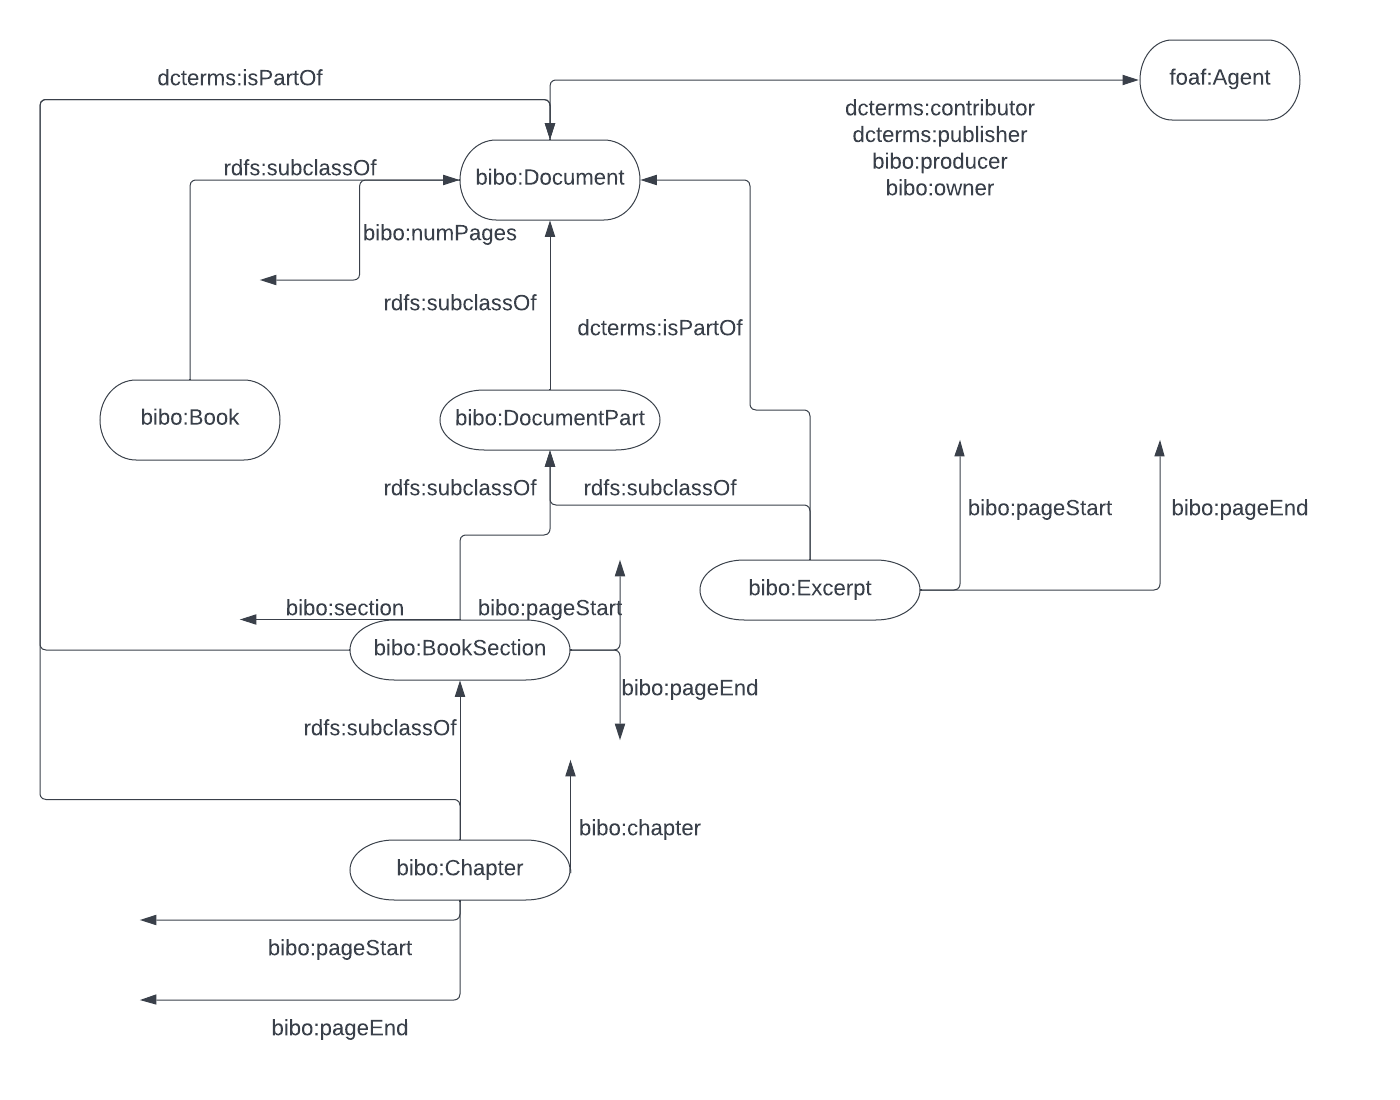
\includegraphics[scale=0.5]{uml-coursematerial.png}
    \end{figure}

    \noindent The classes used to model course materials are \textit{bibo:Book} and \textit{bibo:Document}.
    Which class to use depends on the material: books published by publishers will be modelled with \textit{bibo:Book}.
    If a teacher makes its own material, the class \textit{bibo:Document} should be used.\\ \\
    Course materials are always split up into chapters. Sometimes an author can opt to divide the materials into sections. That's why both \textit{bibo:Chapter} and \textit{bibo:BookSection} are needed.\\
    The class \textit{bibo:Excerpt} represents a small, continuous part of a document. This is used to reference pages of the documents, but can also be used to even further model the structure of the document.
    For example: one could add Excerpts that covers the pages that hold all exercises for a certain chapter.
    Chapters can often be further divided into coherent subject matter. Excerpts can be used to model this as well.\\
    It is up to the creator of the data to decide how detailed the documents are described: this class can be used in a flexible manner.\\ \\
    In the sections that follow, the modelling of course material and exercises is discussed further.\\
    An overview of how this data is modelled can be found in figure \ref{fig:uml-materialdata}.

    \begin{figure}[h]
        \centering
        \caption{Modelling of course materials and exercises}
        \label{fig:uml-materialdata}
        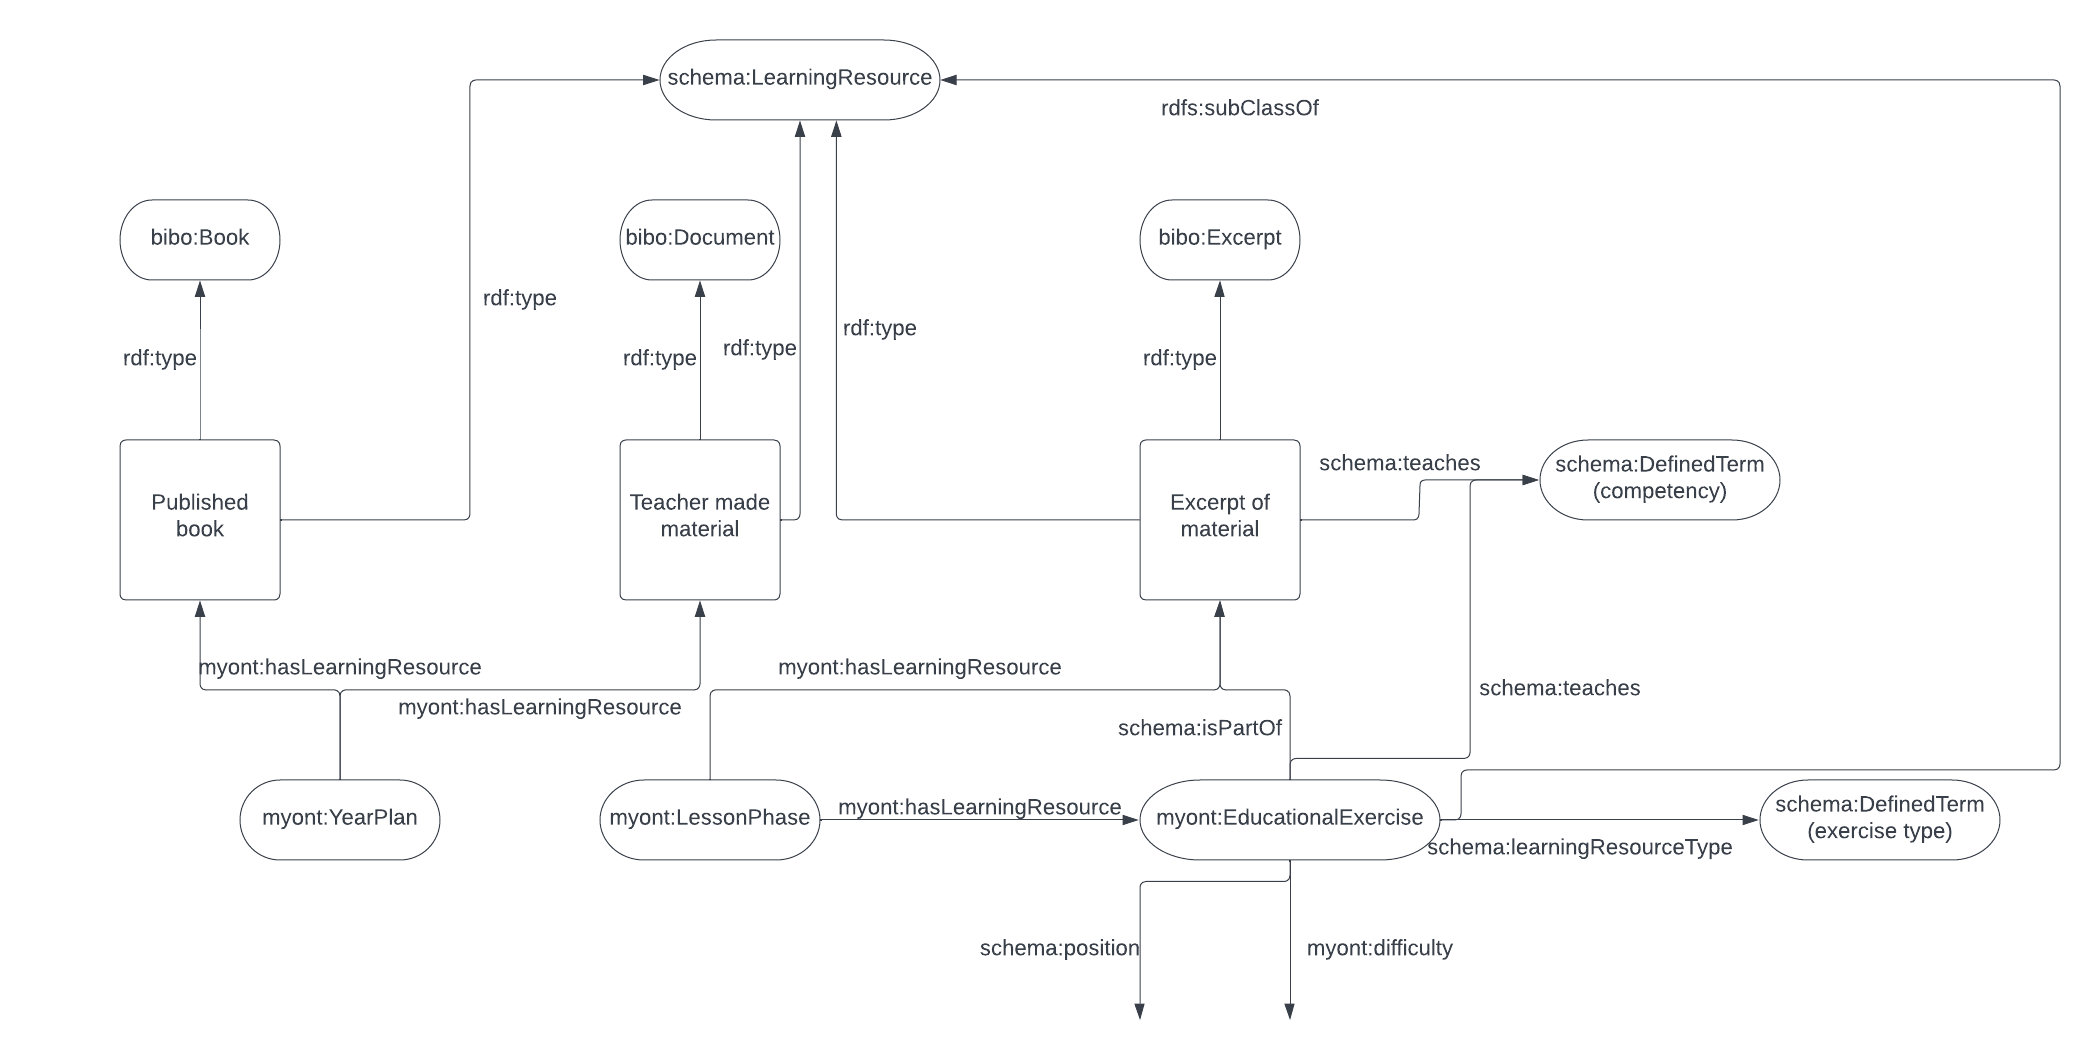
\includegraphics[scale=0.5]{uml-materialdata.png}
    \end{figure}

    \subsection{Course materials}

    As seen in figure \ref{fig:uml-materialdata}, every course material has 2 types: \textit{schema:LearningResource} and \textit{bibo:Document} or a subclass.\\
    This is needed because properties of both the DC ontologies and Schema.org are used to describe course materials.\\
    The documentation for \textit{schema:LearningResource} \footnote{https://schema.org/LearningResource} states that \textit{``LearningResource is expected to be used as an addition to a primary type such as Book, VideoObject, Product etc.''}\\
    This is the reason that \textit{schema:LearningResource} was chosen instead of \textit{schema:CreativeWork}: course materials are books (or documents) that happen to be used for learning.\\
    Another option could have been to add the triple \textit{(bibo:Document rdfs:subClassOf schema:CreativeWork)}, which would semantically be correct (every document is created by someone and thus is a creative work).
    This choice would eliminate the need for 2 triples with \textit{rdf:type} as predicate, which reduces the chance of faulty data.\\
    It was not done this way to keep the model as consistent as possible with the official documentation of both Schema.org and DC.\\ \\
    No new classes are introduced to represent course materials. This is because Schema.org and DC offer enough granularity, in contrast to repsrenting year plannings and all it's aspects (as mentioned in section \ref{subsection:yearplans}).\\
    Important properties concerning course material are the following:
    \begin{itemize}
        \item \textit{dcterms:publisher, dcterms:contributor, bibo:owner and bibo:producer} are used to indicate a person published, contributed to, owns or produced the document.
        This points to a \textit{foaf:Agent} because of their ``good neighbour agreement'' with foaf \cite{dc}.
        \item \textit{dcterms:title} is a string containing the title of the document.
        \item \textit{bibo:references} can be used to give copyright credits to referenced works.
    \end{itemize}
    To model the structure of course materials, the classes \textit{bibo:BookSection}, \textit{bibo:Chapter} and \textit{bibo:Excerpt} are used. They are all subclasses of \textit{bibo:DocumentPart}.\\
    Important properties are the following:

    \begin{itemize}
        \item \textit{bibo:pageStart and bibo:pageEnd} are integers indicating a continuous range of pages of a document or book.
        \item \textit{bibo:chapter and bibo:section} are integers indicating the position of respectively a chapter and section in a document or book.
        \item \textit{dcterms:isPartOf} points to a \textit{bibo:Document} of which this \textit{bibo:DocumentPart} is part of.
    \end{itemize}
    When using \textit{dcterms:isPartOf}, it is useful to have a triple pointing to the URI of the course material.\\
    This allows for simpler queries as opposed to only defining that for example a \textit{bibo:Excerpt} is part of a \textit{bibo:Chapter}.
    The latter could also be added, but increases the risk of inconsistent data. Because this data is not very volatile, one could choose to add these triples depending on the situation. \\
    This is however not needed here because this information can be deduced from the \textit{bibo:pageStart and bibo:pageEnd} properties.\\ \\
    The property \textit{myont:hasLearningResource} was introduced to indicate that course material is used in a creative work.\\
    The domain of this property, \textit{schema:CreativeWork}, is intentionally broad to ensure reusability. This property should only be used on creative works with an educational goal.\\
    That is why the range of this property is \textit{schema:LearningResource}.

    \subsection{Exercises}
    \label{subsubsection:exercises}

    Exercises are modelled by introducing a new class: \textit{myont:EducationalExercise}. Schema already provides classes for physical exercises, hence the need to specify that this exercise is educational.\\ \\
    The class \textit{schema:Question} was not used for two reasons.\\
    The first, and most important, reason is that this class is originally intended for FAQ documents and online platforms.
    As of writing, the property \textit{eduQuestionType} was proposed for questions that are part of learning resources, but not yet accepted.\\
    Another reason is the semantics of the class \textit{schema:Question}: it is a subclass of \textit{schema:Comment} which does not correspond to the semantics of questions in an educational context.\\
    Also, an exercise is not necessarily a question: it could be an instruction or a list of questions/instructions.\\
    One could introduce new classes to offer more granularity of educational questions, but this is outside the scope of this research.\\ \\
    The property \textit{schema:isPartOf} is used to indicate an exercise is part of a learning resource.
    In the data presented with this paper, the values of this property are always URIs to an excerpt because this offers a high degree of granularity.
    Depending on the situation, one might opt to point to a chapter, section or a book.\\ \\
    The property \textit{schema:learningResourceType} is used to indicate the type of exercise. This can be either a string or a \textit{schema:DefinedTerm}.\\
    The \textit{schema:DefinedTerm} was chosen because there is no standardized name for the different types. This can however be a useful search criteria so it is a good idea to keep these types consistent.\\
    That's why a \textit{schema:DefinedTermSet} was defined, containing \textit{schema:DefinedTerm}s representing the different types of exercises.\\ \\
    The property \textit{myont:difficulty} was introduced to represent the difficulty of an exercise, as estimated by the creator of the data.\\
    The possible values are defined in the official vocabulary of the Flemish government \cite{pubelovoc} and are the following:
    \begin{itemize}
        \item ``very easy'' (``Erg gemakkelijk'')
        \item ``easy'' (``gemakkelijk'')
        \item ``medium'' (``gemiddeld'')
        \item ``difficult'' (``moeilijk'')
        \item ``very difficult'' (``Erg moeilijk'')
    \end{itemize}
    Because of this standardized and exhaustive list of options, strings are used rather than \textit{schema:DefinedTerm}.
    Even though the government did release this vocabulary, it will most likely not provide URIs for these values. That's why an atomic datatype was chosen for this.\\
    It is however possible to represent this with \textit{schema:DefinedTerm} with minimal changes.\\
    \textit{schema:educationalLevel} could have been used as well for this, but is already used in the context of educational levels defining which competencies should be acquired.
    Loooking at the official vocabulary of the Flemish government \cite{pubelovoc}, it is expected that properties with this name indeed have to be used for levels in an educational system, not difficulties of execises.\\ \\
    To indicate an exercise is featured in a lesson, instances of \textit{myont:LessonPhase} can have the property \textit{myont:hasLearningResource} pointing to an exercise.
    Instances of \textit{myont:Lesson}, \textit{myont:LessonSeries} and \textit{myont:YearPlan} can also have this property but this would either increase the risk of inconsistencies or reduce granularity.

    \subsection{Results}
    \label{subsection:results}
    In what follows, the problems with existing tools, as mentioned in section \ref{subsection:existingtools}, and how this model eleviates them, are discussed.

    \begin{itemize}
        \item Linking lessons and exercises to the covered competencies can be done with \textit{schema:teaches}.
        \item The data can be decentralized: teachers create lessons, schools create courses, publishers create educational materials and so one. When the servers of one of these actors failed, one can still use other functionality and optionally cache previous results. With good caching, the user might not even notice that servers are down.
        \item This model is compatible with any ontology that a government or official organization uses to communicate competencies.
        \item More insightful information can be offered than only the covered competencies. The competency questions give a good overview of which information can be offered.
        \item Lessons and lesson phases can be linked to the educational material it uses. This can be done on page level if so desired.
        \item Lesson phases were introduced to increase granularity. This enables teachers to easily move around parts of lessons to different lessons.
        \item Because of the decentralized nature, information comes from different sources. Teachers can for example rely on metadata created by a publisher to decide which pages are taught in which lessons.
    \end{itemize}
    Decoupling lessons (without temporal data) from classes, offers flexibility to treat the year planning as a dynamic instrument, which is needed according to the interviewees (see section \ref{subsection:interviews}).


    \section{Didactical methods and educational taxonomies}
    \label{subsection:taxonomies}
    Lastly, the modelling of didactical methods and educational taxonomies is discussed.\\
    The used properties and classes to model this can be found in figure \ref{fig:uml-dm}.

    \begin{figure}[h]
        \caption{Modelling of didactical methods and taxonomies}
        \label{fig:uml-dm}
        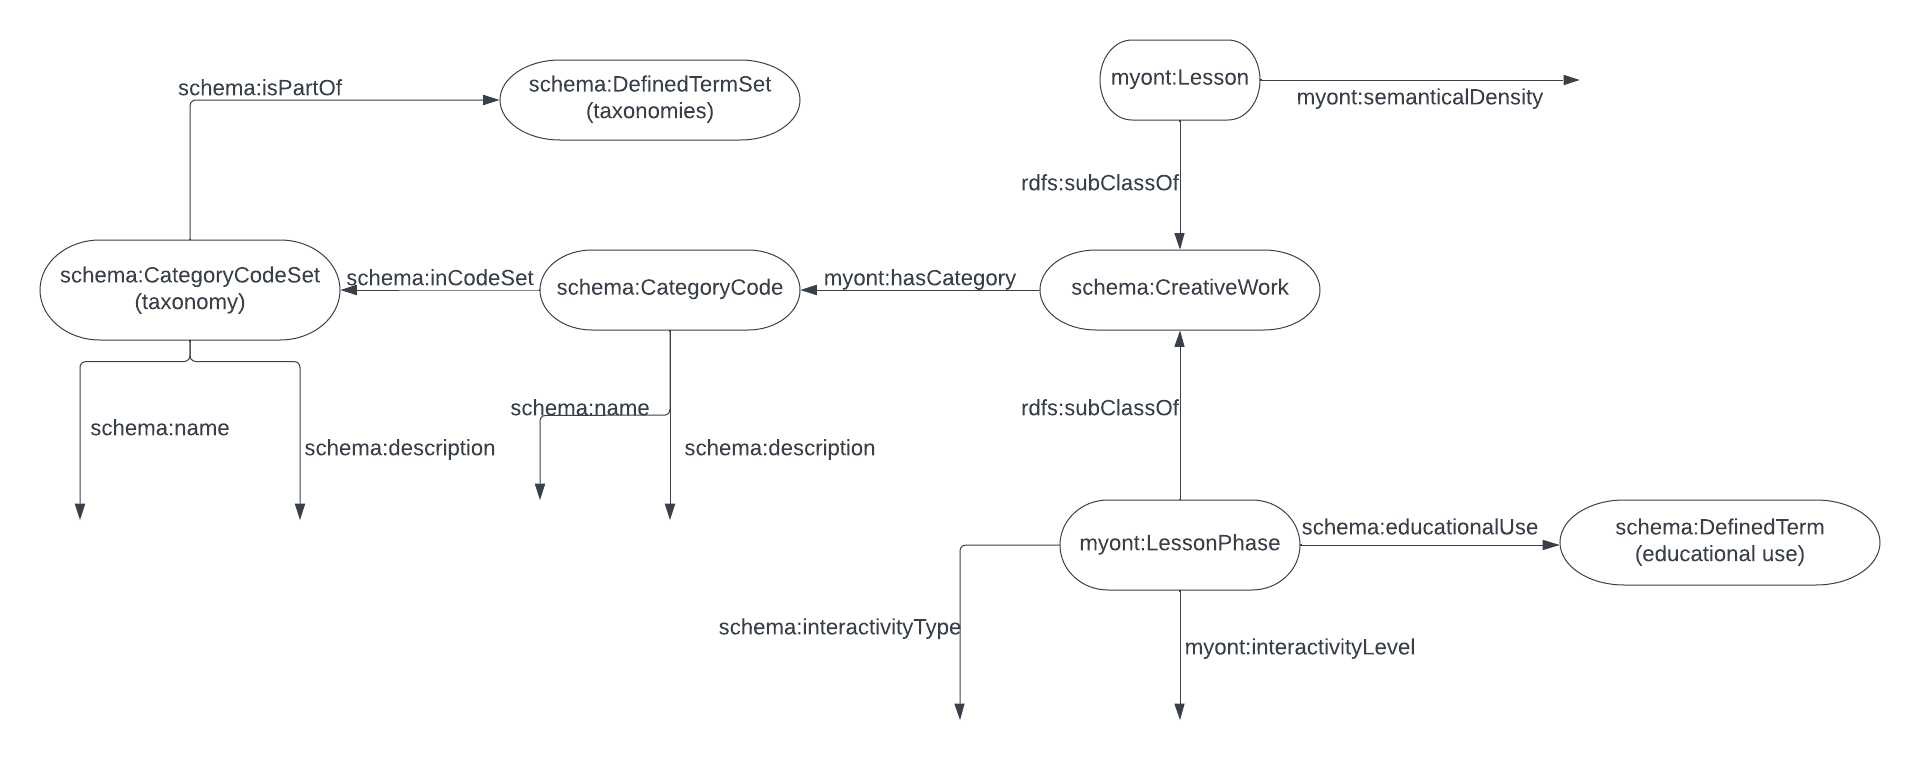
\includegraphics[scale=0.5]{uml-taxonomies.png}
    \end{figure}

    \subsection{Didactical methods}
    Didactical methods are not represented by a seperate class in this model. Representing whole didactical methods is a research of its own and thus outside the scope of this paper.\\
    The choice was made to add properties to the existing classes representing the important characteristics of didactical methods, as mentioned in section \ref{subsection:interviews}.
    The reason behind this is to be sure that teacher have to put in as less data as possible.\\
    Some didactical methods can be used with different intentions.
    For example an exercise lesson can have as goal to remediate, introduce new subject matter or rehearse already taught subject matter.\\
    For this use case, it is not important what the name of the didactical method is or what its general uses are.
    That's why the important characteristics are modelled as properties of the existing classes representing lessons and lessonp hases.\\
    These properties are the following:
    \begin{itemize}
        \item \emph{schema:interactivityType} indicates the type of interactivity of a lesson phase as a string. Following the vocabulary of the Flemish government \cite{pubelovoc}, possible values are the following:
        \begin{itemize}
            \item ``active'' (``actief'')
            \item ``expositive'' (``receptief'')
            \item ``mixed'' (``gemengd'')
        \end{itemize}
        \item \emph{myont:interactivityLevel} represents the level of interactivity of a lesson phase as a string. Following the vocabulary of the Flemish government \cite{pubelovoc}, the possible values are the following:
        \begin{itemize}
            \item ``Very low'' (``Erg laag'')
            \item ``low'' (``laag'')
            \item ``medium'' (``gemiddeld'')
            \item ``high'' (``hoog'')
            \item ``Very high'' (``Erg hoog'')
        \end{itemize}
        \item \emph{schema:educationalUse} has as value a string or a \textit{schema:DefinedTerm} representing the use of a lesson phase. A set of possible uses was made to keep consistency (see further)
        \item \emph{myont:semanticalDensity} represents how much subject matter is handled in a lesson, as estimated by the teacher creating the data. The values are strings that follow the official vocabulary \cite{pubelovoc}. Possible values are the following:
        \begin{itemize}
            \item ``Very low'' (``Erg laag'')
            \item ``low'' (``laag'')
            \item ``medium'' (``gemiddeld'')
            \item ``high'' (``hoog'')
            \item ``Very high'' (``Erg hoog'')
        \end{itemize}
    \end{itemize}
    The reason for choosing atomic datatypes and not \textit{schema:DefinedTerm} for these properties (except \emph{schema:educationalUse}) is analogous to difficulty of exercises, mentioned in section \ref{subsubsection:exercises}.

    \subsection{Educational taxonomies}
    Taxonomies are modelled using the classes \textit{schema:CategoryCodeSet} (for a taxonomy) and \textit{schema:CategoryCode} (for a category of a taxonomy).\\
    As of writing, these classes were proposed to be added to schema, but not yet accepted. These classees do however semantically correspond with taxonomies.\\
    The classes \textit{schema:DefinedTerm}  and \textit{schema:DefinedTermSet} could have been used as well, but these relate less to taxonomies than the used classes.\\ \\
    To easily access all taxonomies, a \textit{schema:DefinedTermSet} was used.\\
    Important properties are the following:
    \begin{itemize}
        \item \emph{schema:name and schema:description} represent the name and description of the taxonomy/category as string.
        \item \emph{schema:codeValue} is a textual code identifying a catgory. This should be unique at least across all categories of the same taxonomy.
        \item \emph{schema:inCodeSet} indicates that a category is part of a taxonomy.
        \item \emph{myont:hasCategory} points to a \emph{schema:CategoryCode} representing the category of a creative work (usually a lesson phase or exercise).
    \end{itemize}
    The property \textit{myont:hasCategory} was introduced because, as of writing, Schema.org does not provide a property linking a creative work with a category.
    When Schema.org does introduce this, \textit{myont:hasCategory} should be replaced by the property proposed by Schema.org to maximize interoperability.

    \subsection{Results}
    In what follows, the problems with existing tools, as mentioned in section \ref{subsection:existingtools}, and how this model eleviates them, are discussed.

    \begin{itemize}
        \item Linking lessons and exercises to the covered competencies can be done with \textit{schema:teaches}.
        \item The data can be decentralized: teachers create lessons, schools create courses, publishers create educational materials and so one. When the servers of one of these actors failed, one can still use other functionality and optionally cache previous results. With good caching, the user might not even notice that servers are down.
        \item This model is compatible with any ontology that a government or official organization uses to communicate competencies.
        \item More insightful information can be offered than only the covered competencies. The competency questions give a good overview of which information can be offered.
        \item Lessons and lesson phases can be linked to the educational material it uses. This can be done on page level if so desired.
        \item Lesson phases were introduced to increase granularity. This enables teachers to easily move around parts of lessons to different lessons.
        \item Because of the decentralized nature, information comes from different sources. Teachers can for example rely on metadata created by a publisher to decide which pages are taught in which lessons.
    \end{itemize}
    Decoupling lessons (without temporal data) from classes, offers flexibility to treat the year planning as a dynamic instrument, which is needed according to the interviewees (see section \ref{subsection:interviews}).


    \chapter{Data}
    \label{section:data}
    To prove that this is a functional model, and to test the SPARQL queries, a number of data files were created. This was made available as Turtle-files in the GitHub repository \cite{repo}.\\
    Data was generated for all concepts that are being modelled. It consists of randomly generated data and `real' data. This is data that came from real life and realistic sources.\\ \\
    The data describing the newly introduced classes and properties, can be found in appendix \ref{chap:appendix-myont}.
    In the coming sections, the created data is discussed. It is split up into parts similar to section \ref{section:datamodelling}.

    \section{Competencies, credentials, educational levels and domains}
    \label{subsection:comp}
    The data concernig competencies are based on the data of the Ilearn project \cite{ilearnskosmos}.
    This was created by hosting a SPARQL-endpoint on the data of Ilearn and running SPARQL CONSTRUCT queries to parse the data to the model discussed in this paper.\\
    The Python code can also be found in the repository. This code is a good reference for people wanting to use this model.\\
    The resulting files are the following:
    \begin{itemize}
        \item \emph{comp.ttl} models the competencies of the Flemish educational system.
        \item \emph{domain.ttl} are all domains and subdomains of which a competency can be part of.
        \item \emph{eduLevels.ttl} models the educational levels that a pupil can choose from.
        \item \emph{cred.ttl} contains data concerning the credentials that can be acquired.
    \end{itemize}

    \section{Real lessons}
    In the folder \emph{real-data} in the repository, turtle files can be found that represent real lessons that were taught to pupils in Flanders.
    This folder consist of following files and subfolders:
    \begin{itemize}
        \item \emph{lessen.ttl} contains the instances of myont:Lesson.
        \item \emph{lesfasen.ttl} contains the instances of myont:LessonPhase.
        \item \emph{documents.ttl} contains instances of schema:DigitalDocument and represent markdown documents describing the lesson phases.
        \item \emph{documents} is a folder containing the markdown documents that describe the lesson phases.
    \end{itemize}
    These `real' lessons do not contain data about the goals they cover.
    This is because teachers in Flanders don't base their lessons on competencies set by the government.
    Instead, there are official organizations (`Onderwijskoepels') that create curricula based on the competencies set by the government.
    It are these curricula that have to be taught instead of the competencies set by the government.\\
    These curricula are not part of this paper, but can be modelled in the same way as competencies are modelled now.\\ \\
    Data about lesson phases covering competencies is present in the generated lessons (see section \ref{subsection:generated-lessons}).

    \section{Generated year plan}
    \label{subsection:generated-lessons}

    The Python script \emph{generate-yearplan.py} generates a yearplan and saves all data in turtle files per class.\\
    The year plan is generated as follows: 

    \begin{enumerate}
        \item Select all competencies that are required for the chosen credential and put them in an array.
        \item Create a year plan.
        \item Create 3-6 lesson series.
        \item For every lesson series, generate 5-15 lessons.
        \item For every lesson, generate 6-10 lesson phases.
        \item For every lesson phase:
            \begin{enumerate}
                \item create a markdown document,
                \item add rdf-data representing the markdown document,
                \item select 0-3 competencies,
                \item add all data about the lesson phase to the graph.
            \end{enumerate}
        \item Write all graphs to seperate turtle files.
    \end{enumerate}
    It is important to mention that the only logical coherence is that all competencies are required for the same credential.
    The order in which the competencies are taught is not logical nor practical, they are just randomly selected.\\ \\
    This data is the core data to test the SPARQL queries concerning lessons.\\
    It shows that it is possible to model lessons and year plannings, keeping the problems mentioned in section \ref{subsection:goals} in mind.
    The SPARQL queries answering the competency questions can be ran on this data and they result in correct answers.\\
    This means that the model is functional and could be used to model year plannings.
    \subsection{Generated courses, subjects and classes}
    The script \emph{create-course.py} creates a course with two subjects. The subjects differ in school year and have different schedules.
    For every subject, all classes are generated. Some classes have the \emph{schema:workPerformed} property, but not all of them.
    This is a realistic scenario: a teacher will not plan all lessons at once for a whole school year.\\ \\
    This script is a good reference if one would like to use this model.
    It shows how Python can be used to generate all dates and hours on which classes occur, given the data about the schedule as discussed in section \ref{subsubsection:subject}.\\ \\
    The official holidays in Flemish education are incorporated, but not the vacations.\\
    The resulting turtle files are found in the folder \emph{rdf-data/generated-data} and are called \emph{generated-courses.ttl, generated-subjects.ttl, generated-classes.ttl and generated-schedules.ttl}.
    Excerpts of the generated lessons and phases can be found respectively in appendix \ref{chap:appendix-lesson} and appendix \ref{chap:appendix-phase}.

    \subsection{Course material, exercises, didactical methods and taxonomies}
    To test the part of the model concerning course material and exercises (section \ref{subsection:coursematerial}), data was created based on materials that are used in a Flemish school.\\
    There is a book, created by a publisher, and a document created by a teacher that was based on this book.
    The titles were changed to avoid copyright issues.\\ \\
    The data was created by first representing the materials as a JSON file containing the chapters (name and pages) and excerpts (name, pages and exercise numbers).\\
    These excerpts are either the different theoretical parts of a chapter, or the exercisese of a chapter.\\ \\
    These JSON files are then parsed to turtle data and random data for the covered competencies of excerpts and exercises and difficulty of exercises was added.\\ \\
    The choice was made to only add data to represent covered competencies for excerpts, and not chapters, for optimal granularity without the risk of inconsistent data.\\
    The creator of the data can choose how granular it wants this data to be.\\
    The code for this can be found in the repository \cite{repo} in the file \textit{create-coursematerials-and-exercises.py}.
    This is good reference code if one wishes to represent its own material using this model. The JSON model can be modified depending on the needs of the creator.\\ \\
    Linking the course materials to the lessons is done in \textit{link-lessons-documents.py}.\\
    These links are only made on phase level to ensure consistency and granularity.
    Only one excerpt per phase is added. This is a realistic scenario as phases should be as small as possible. Going to a new part of the course material could be seen as a new phase.\\
    One could link multiple excerpts to a single phase, depending on the situation.\\
    Note that this is completely randomized: excerpts will belong to only one chapter, but which chapter is completely randomized.\\ \\
    Lastly, didactical methods and taxonomies are added to the lessons and exercises in the script \textit{didactical-methods-and-taxonomy.py}.\\
    All data for this is completely randomized.\\

    \chapter{Conclusion}
    \label{section:conclusion}
    This research is twofold: it identifies the needs of teachers for maintaining year plannings, and develops a model meeting those needs.\\ \\
    To start, interviews were conducted with teachers that have some experience. The main goal of this was to find out how teachers keep track of their year plannings, and what they think they're missing.\\
    Important properties of lessons and didactical methods were identified, and useful features were proposed (as described in section \ref{subsection:interviews}). These were the basis for developing the model.
    The interviews were processed into requirement stories and these were further processed into competency questions and contextual statements, following the principles of eXtreme Design \cite{xd}.\\ \\
    All competency questions have a corresponding SPARQL query, as can be found in the acoompanying repository \cite{repo}. This implies that it is possible to create a model that meets the input of the interviewees.\\ \\
    At all times consistency and granularity were prioritized, making the queries sometimes more difficult. For example excerpts are bound to phases, rather than lessons.
    This makes it harder to find out which pages were taught in a lesson, but does increase consistency and granularity.\\
    Future data creators using this model, can deviate from this if they deem this a better option.\\
    The model is created in such a way that flexibility is possible. For example, documents can describe phases, lessons or lesson series.\\
    This enables reusing existing documents: if teachers already created documents describing complete lessons, these can be reused. More granular metadata can still be added to enable useful insights.\\ \\
    There was also a strong focus on reusing existing ontologies rather than creating new ones. The model mostly uses Schema.org and DC, as mentioned in section \ref{subsection:ontologies}.\\
    Some new properties and classes were introduced when the existing ontologies didn't suffice. These choices were always motivated.

    \chapter{Future work}

    This work opens the possibility for creating tools helping teachers maintaining year plannings.
    Multiple tools would be needed: teachers making lessons, schools making schedules, publishers annotating their course materials and so on.\\
    These tools would rely on each others data, following the principles of the semantic web.\\ \\
    Representing the structure of schools was out of scope for this research, but is important to create tools using this data model.
    This model could include the staff of the school, its pupils, its location and other spatial information, special days like school trips and so on.\\ \\
    As mentioned in section \ref{subsubsection:exercises}, there is not a lot of granularity representing exercises. This could be further developed with compound exercises, exercise series, exercises relying on others...\\
    Also tests and exams could be added.\\ \\
    A more refined model for didactical methods can be of use to inspire teachers to use new methods. Some research about this has already been done \cite{hierarchy}, but no usable RDF ontologies have been developed for this.
    This is especially useful for lessons with high interactivity.\\ \\
    Representing subject matter in more detail can be useful, especially for artificial intelligence. Chimalakonda, S. et al \cite{dida} propose a very detailed, yet flexible, ontology for this.
    This ontology models instructional design. This is very closely related to lessons, but not quite the same. Linking this model with the model of this paper can enable powerful AI systems.\\ \\
    Teachers will often differentiate within a lesson. A group of pupils can be quite diverse and a teacher should incorparate this in its lessons.
    Modelling differentation is not explicitly part of this model, but it can be done by mentioning differentiation in the \textit{schema:description} property or in the describing document. 
    Distinguishing mandatory exercises from optional exercises is a good example of differentiation that is not explicitly part of this model, but can be acquired. \\ \\

\bibliographystyle{IEEEtran}
\bibliography{bibliography}
% \printbibliography

\appendix
\chapter{Competency questions regarding didactical methods and taxonomies}
\label{chap:appendix-cq}
\VerbatimInput{../competency-questions/didactical-methods-and-taxonomies.md}

\chapter{Self defined classes and properties}
\label{chap:appendix-myont}
\VerbatimInput{../rdf-data/myont.ttl}

\chapter{Excerpt of turtle data with generated lessons}
\label{chap:appendix-lesson}
\VerbatimInput{excerpt-lessons.ttl}

\chapter{Excerpt of turtle data with generated phases}
\label{chap:appendix-phase}
\VerbatimInput{excerpt-phases.ttl}

\end{document}